\documentclass[12pt,a4paper,bold]{thesis}

% ------------------------------
% Information on how to use this file
% ------------------------------
%
% This file was prepared under the MikTex distribution <http://miktex.org/>
% All packages such as "thesis", "amsmath", "graphicx", "epstopdf", etc. are available on <http://ctan.org/>.
% Most Latex editors (such as WinEdt/TexMaker/Texniccenter) will download these for you as you try to compile this file.
% Please change the Individual Details below before you compile.
% The following pages are optional. You can comment out the corresponding lines before compiling :
% - List of Symbols
% - Appendix
%
% Note: Often, you will have to compile the file twice to see the changes correctly. This is because of the way the \tableofcontents command works.
%
% In case of any questions, please contact Dr. Prahlad Vaidyanathan <prahlad@iiserb.ac.in>

% ------------------------------
% Preamble
% ------------------------------

\usepackage{amsmath}
\usepackage{amsthm}
\usepackage{amssymb}
\usepackage{setspace}
\onehalfspacing

\usepackage[pdftex]{hyperref}
\hypersetup{colorlinks,
                        citecolor=blue,
                        filecolor=blue,
                        linkcolor=blue,
                        urlcolor=blue}

                        
\usepackage{caption}
\usepackage{subcaption}

\usepackage{float}
\usepackage{graphicx}
\usepackage{epstopdf}

\usepackage[toc, page]{appendix}

\theoremstyle{thm}
\newtheorem{thm}{Theorem}[chapter]
\theoremstyle{definition}
\newtheorem{exmp}[thm]{Example}
\newtheorem{defn}[thm]{Definition}
\newtheorem{rem}[thm]{Remark}

\providecommand{\appendixname}{Appendices}
%\newcommand{\appendixtocname}{Appendices}
%\newcommand{\appendixpagename}{Appendices}

\newcommand{\head}[1]{\newpage
\vspace{3em}
\begin{center}
\LARGE{\MakeUppercase{\textbf{#1}}}
\end{center}
\vspace{3em}
\addcontentsline{toc}{chapter}{#1}
}
\renewcommand{\listfigurename}{}
% ------------------------------
% Individual details (Change these!)
% ------------------------------

\newcommand{\thesistitle}{Neuromorphic hardware design}
\newcommand{\studentname}{Khritish Kumar Behera}
\newcommand{\studentrollno}{17125}
\newcommand{\advisorname}{Dr. Kuntal Roy}

\newcommand{\degreename}{BS-MS}
\newcommand{\subject}{Electrical Engineering and Computer Science}
\newcommand{\thesisdate}{April 2022}

% ------------------------------
% Title page
% ------------------------------

\def\maketitle{
\begin{titlepage}
\begin{center}
\begin{doublespace}
\textbf{\MakeUppercase{\LARGE{\thesistitle}}} \\
%\ \\
\ \\
\normalsize{\textbf{A THESIS}} \\
\normalsize{\textit{submitted in partial fulfillment of the requirements}} \\
\normalsize{\textit{for the award of the dual degree of}} \\
%\ \\
%\ \\
\large{\textbf{Bachelor of Science-Master of Science}} \\
\normalsize{\textit{in}} \\
\large{\textbf{\MakeUppercase{\subject}}} \\
\normalsize{\textit{by}} \\
\large{\textbf{\MakeUppercase{\studentname}}} \\
\normalsize{\textbf{(\studentrollno)}} \\
% \normalsize{\textit{Under the guidance of}} \\
% \large{\textbf{\MakeUppercase{\advisorname}}}
\end{doublespace}
\vfill
\centerline{
\includegraphics[scale=0.20]{iiser_b.png}}
\ \\ 
\textbf{DEPARTMENT OF \MakeUppercase{\subject} \\ 
INDIAN INSTITUTE OF SCIENCE EDUCATION AND RESEARCH BHOPAL\\ %Flows onto two lines
BHOPAL - 462066} \\ 
\ \\
\textbf{\thesisdate}
\end{center}
\end{titlepage}
}

% ------------------------------
\begin{document}
\maketitle

\pagenumbering{roman}

% ------------------------------
\head{Certificate}

This is to certify that {\bf \studentname}, BS-MS (\subject), has worked on the project entitled {\bf `\thesistitle'} under my supervision and guidance. The content of this report is original and has not been submitted elsewhere for the award of any academic or professional degree.

\vspace{10em}

\textbf{\thesisdate \hfill \advisorname \\ IISER Bhopal}

\vfill

\begin{center}
\begin{tabular}{ccc}
\textbf{Committee Member} & \textbf{Signature} & \textbf{Date} \\
\\
\rule{15em}{0.4pt} & \rule{10em}{0.4pt} & \rule{6em}{0.4pt} \\
\\
\rule{15em}{0.4pt} & \rule{10em}{0.4pt} & \rule{6em}{0.4pt} \\
\\
\rule{15em}{0.4pt} & \rule{10em}{0.4pt} & \rule{6em}{0.4pt} \\
\end{tabular}
\end{center}

% ------------------------------
\head{Academic Integrity and Copyright Disclaimer}

I hereby declare that this project is my own work and, to the best of my knowledge, it contains no materials previously published or written by another
person, or substantial proportions of material which have been accepted for the award of any other degree or diploma at IISER Bhopal or any other educational
institution, except where due acknowledgement is made in the document. \\

I certify that all copyrighted material incorporated into this document is in compliance with the Indian Copyright Act (1957) and that I have received written permission from the copyright owners for my use of their work, which is beyond the scope of the law. I agree to indemnify and save harmless IISER Bhopal from any and all claims that may be asserted or that may arise from any copyright violation.

\vfill

\textbf{\thesisdate \hfill \studentname \\ IISER Bhopal}

% ------------------------------
\head{Acknowledgement}

I would like to express my warmest thanks to my advisor Dr. Kuntal Roy for allowing me to work on this project. His advice and guidance carried me through all the stages of this project.\\\\ 
I would also like to thank Mohanlal Naik for taking time out of his busy schedule and providing me with valuable insights. I thank my colleagues Keshav Bihani, Nitanshu Bhagawat Kate, and Lakhvir Singh for their vital aid and discussions. I want to thank the IISER Bhopal community for providing a lively atmosphere full of enthusiasm for Science. \\
Finally, I would like to thank my mother, grandfather, and the whole family for the support and moral guidance that kept me motivated to pursue my dreams. 

\vspace{7em}

\begin{flushright}
    {\bf \studentname}
\end{flushright}

% ------------------------------
\head{Abstract}

We have gone far faster in terms of computation than our human brain. But biological systems have
some distinct capabilities like recognizing faces from the crowd, even when wearing a mask. Biological systems
require very little power to operate. The ultimate solution for low-power brain-inspired computing is to replicate
the neural architecture of the brain on a chip. The aim of the project is to design and fabricate neuromorphic
spin-devices using multiferroics exploiting its novel spintronic device concepts. As a proof-of-concept we plan
to implement a character recognition system using back-propagation neural network algorithm.


% ------------------------------
\head{List of Symbols or Abbreviations}

\begin{center}
\begin{tabular}{l@{\hspace{7em}}l@{}} \smallskip
	$\alpha$ & The first letter \\ \smallskip
	$\omega$ & The last letter \\ \smallskip
	$\zeta(s)$ & The Riemann Zeta function \\ \smallskip
\end{tabular}
\end{center}

% ------------------------------
\head{List of Figures}
%\begin{center}
%\begin{tabular}{l@{\hspace{7em}}l@{}} \smallskip
%	Not a function & 2 \\ \smallskip
%\end{tabular}
%\end{center}
%\clearpage
\listoffigures

%\phantomsection
%\addcontentsline{toc}{chapter}{List of Figures}
%\listoffigures
%\cleardoublepage

% ------------------------------
\head{List of Tables}
\begin{center}
\begin{tabular}{l@{\hspace{7em}}r@{}} \smallskip
	Nonlinear Model Results & 5 \\ \smallskip
\end{tabular}
\end{center}
%\listoftables
\tableofcontents

% ------------------------------
\chapter{Introduction} \label{ch: introduction}
\pagenumbering{arabic}

% ------------------------------
%\section{Basic Introduction}
Spin-electronics or so-called spintronics is a rapidly developing nanotechnology. Spintronic
devices can be used to store, process, and communicate information. They also possess in-built functionalities for performing certain tasks efficiently. Spintronic devices can be energy-efficient than the transistor-based devices since there is no charge movement causing Ohmic dissipation.~\cite{khr123}\\ 
\\
In 2007, Albert Fert and Peter Grunberg were jointly awarded the Nobel Prize in Physics for the discovery of giant magnetoresistance (GMR) back in 1980s, signifying its remarkable transition from fundamental studies to a critical device technology. For the tunneling magnetoresistance (TMR), instead of a metallic spacer, an insulator is used, which boosts the magnetoresistance more than GMR. Here, we will utilize TMR for sensing the magnetization direction.\\
\\
Brain-inspired neuromorphic computing is intended to mimic our brains' working principles~\cite{yon1958computer}~\cite{poon2011neuromorphic}. Biological neural network is a dense network of interconnected neurons which allows them to compute in parallel. An artificial neural network (ANN) models our brains’ neural architecture. ANN is composed of neurons, which performs two basic tasks: Summation of the weighted inputs and applying the activation function on the summed input depicting the firing of a neuron. In the training phase, ANN is trained to get the optimizing parameters of weights and bias. In the evaluation phase, we expect the ANN to perform the desired task with unknown inputs. The target is to build such neuromorphic chip using the novel spintronic device concepts.~\cite{khr124,khr125}
   
% -----------------------------
\section{Artifical Neural Networks (ANNs)}
 An artificial neural network is a collection of interconnected neurons represented as nodes, similar to the biological neural network. Mimicking its biological counterpart, the artificial neuron accepts multiple inputs from other connected neurons by means of an edge. Each edge has a strength associated with it known as \textbf{Weight}, $W$. The weight is one of the two optimizing parameters of the neural network.\\
\\
Each neuron processes through a series of sequential steps, which are represented as \textbf{Summation block} and \textbf{Activation block}. A neuron also possesses the other optimizing parameters of the neural network known as \textbf{Bias} term, $b$.
The summation block performs the summation of the weighted input and the bias term.
%\[\text{Summation block output}=\Sigma_nX_nW_n + b\]
The output of the summation block is fed into the activation block. The output of the activation block is the final output of the neuron.\\
\\
The working of a neural network is a two-phase process: \textbf{Training}, and \textbf{Evaluation}. In the training phase, the neural network (NN) is trained on training data. Training data is a tuple $(X, T)$, where X is the input and T is the desired output or target. The training data is fed into the NN, and the model learns the underlying feature of the data and optimizes its weight and biases, so as to obtain a minimum error. Then comes the evaluation phase, where the trained NN is used to obtain the output for those inputs, for which the network was never trained for.~\cite{khr126}

\begin{figure}[H]
	\centering
   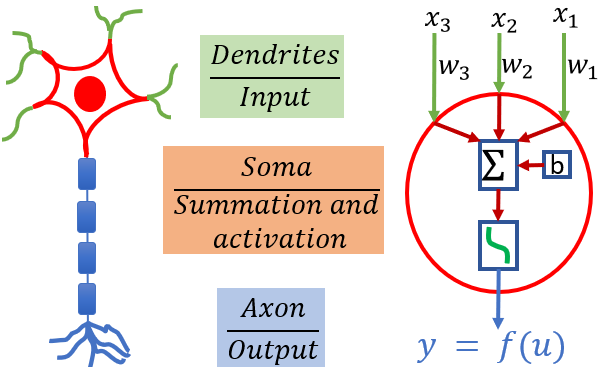
\includegraphics[scale=0.56]{Images/30.png} 
   \caption{Biological neuron vs Artificial neuron }
\end{figure}
\subsection{Architecture}
In an ANN, all the neurons are connected in a specific architecture, the neural architecture. 
The architecture can be viewed as three-layered:\textbf{Input layer}, \textbf{Hidden layers}, and the \textbf{Output layer}.\\
\\
\textbf{Input Layer:}
This layer serves as the input interface between the neural network and the user. The nodes in this layer receive input from the user and send it to its subsequent layers. The nodes in the input layer do not have the bias term. The number of nodes in this layer is dictated by the problem at hand. \\
\\
\textbf{Hidden Layers:}
The hidden layer can be more than one layer. This layer resides between the \textbf{Input layer} and the \textbf{Output layer}. The majority of the computation in an ANN occurs in this layer.  
Since the users do not interact with this layer, hence it is termed the hidden layer.\\
\\
\textbf{Output Layer:}
This layer serves as the input interface between the neural network and the user. The nodes in this layer provide the final output to the user. The number of nodes in this layer is dictated by the problem in hand\\\\
The following rules how a node is connected to another node
\begin{itemize}
	\item No node should be connected to another node in the same layer
	\item There should be no self loop
	\item A node should be connected to all other nodes in the next layer
	\item No node should connect to an another node from the previous layer

\end{itemize}
\begin{figure}[H]
	\centering
   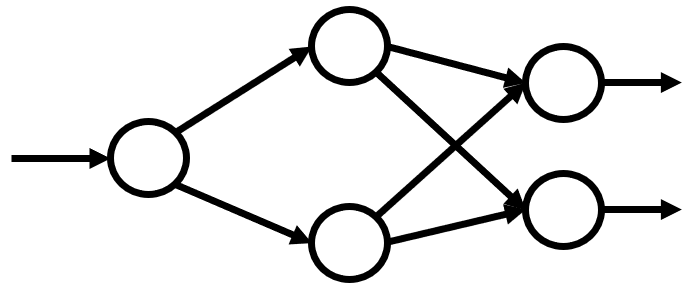
\includegraphics[scale=0.56]{Images/35.png} 
   \caption{ANN architecture }
\end{figure}

\subsection{Activation Function}
The activation function is a non-linear mathematical function. It is the only non-linear component in the whole network. The activation function reflects the activation of a biological neuron in a biological neural network. A biological neuron activates or fires only when the input received reaches a certain threshold. This threshold is the biological counterpart of the bias term in an artificial neuron. The most simplistic activation function is a step function.\\\\
\textbf{Step function}
\[
\text{step}(x)=
\begin{cases}
	1 & \text{if } x>0\\
	0 & \text{if } x\leq0
\end{cases}
\]
In general, a smoother version of the step function is used as an activation function known as the Sigmod function.\\\\
\textbf{Sigmoid function}
\[\text{sigmoid}(x)=\frac{1}{1+e^{-x}}\]
In Deep neural networks, the number of neurons will be in the millions. Using the sigmoid activation function will be computationally expensive for a larger number of neurons. Hence a computationally inexpensive activation function is deployed known as the Rectilinear Unit function (Relu).\\\\
\textbf{Rectilinear Unit function (ReLu)}
\[
\text{ReLu}(x)=
\begin{cases}
	x & \text{if } x>0\\
	0 & \text{if } x\leq0
\end{cases}
\]


\subsection{Forward Propagation}
In Forward-propagation, we need to set our neural architecture, after which the input traverses from the input layer to the output layer through the hidden layers. The weight and bias terms have already been configured. Here is an example: we have taken a very simple ANN with one neuron in the input layer, one in the output layer, and one hidden layer which consists of one neuron. With weights, $W_1$ and $W_2$, for edges connecting \textbf{Node 1} with \textbf{Node 2} and \textbf{Node 2} with \textbf{Node 3} respectively. $X$ is the input given to the NN and $Y$ is the output received from the NN. \textbf{Node 2} and \textbf{Node 3} have the bias term \textbf{$B_2$} and \textbf{$B_3$} respectively. The following figure describes the neural architecture.

\begin{figure}[H]
	\centering
   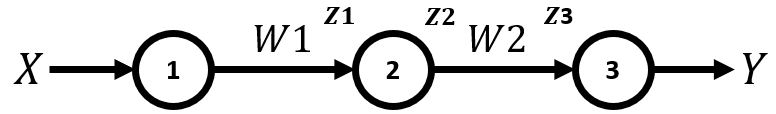
\includegraphics[scale=0.56]{Images/34.png} 
   \caption{Forward propagation }
\end{figure}

Generally, the input node does not have any bias term, it's just a simple node, which accepts input and sends it to its subsequent connected node.\\ 
\textbf{Forward propagation steps:}\\
\begin{itemize}
	\item Input $X$ is provided at the input node, \textbf{Node 1}
	\item Node 1 simply transmits the input to the next node, \textbf{Node 2} through the edge with weight $W_1$ 
	\item Input received by node 2 is $Z_1 = X\cdot W_1$ 
	\item Node 2 process the input $Z_1$ and produces the output $Z_2=\sigma(Z_1+b_2)$, where $b_2$ is the bias term of node 2 and $\sigma$ is the activation function
	\item $Z_2$ is transmitted to \textbf{Node 3} via the edge with weight $W_2$
	\item Input received at Node 3 is $Z_3$, $Z_3=Z_2 \cdot W_2$
	\item Node 3 process the input $Z_3$, and produces the final output of the neural network $Y$, $Y=\sigma(Z_3 + b_3)$
\end{itemize}
\[Y=\sigma(Z_3 + b_3)=\sigma(Z_2 \cdot W_2 + b_3)=\sigma(\sigma(Z_1+b_2) \cdot W_2 + b_3)\]
\[Y=\sigma(\sigma(X\cdot W_1+b_2) \cdot W_2 + b_3)\]
Output from node 1, X

\subsection{Gradient Descent}
Gradient descent is an approach by which the neural network trains itself by minimizing the error in changing the weights and biases accordingly.

In the figure above, we have plotted \textbf{Error} on the y-axis for different values of an \textbf{optimizing parameter, K}. The optimizing parameter can be any weight or any bias term in the neural network. The aim is to choose a value for K such that the error is minimum. \\
To begin with, the initial value of K is chosen randomly. The input is traversed through the neural network using the forward propagation method, from which the error is calculated. The slope at that point is computed, which suggests whether to increase or decrease the value of K inorder to minimize the error and the rate at which the error minimum should be reached. The magnitude of the slope is usually high, hence a \textbf{learning rate, LR} factor is multiplied with the slope. The LR is usually chosen small, but not too small. By multiplying the LR with the slope the step size is computed, which dictates how much large or small jump should K take.
The step size ensures that when K is far away from the minimum, it take larger step size, and when K is near to a minimum, it take smaller step size, in order to avoid overshooting. 
\[\text{Step size} = LR \cdot slope\]
The new value of K is calculated as
\[K_{new}=K - \text{Step size}\]  
\[K_{new}=K - LR \cdot slope\]
\[K_{new}=K - LR \cdot \frac{\partial Error}{\partial K}\]


The initially value of K is chosen randomly for the gradient descent process, the reason for doing so is, if the Error vs K plot turns out to have a lot of local minima. And if we always start from a fixed point, then there is a heavy chance, it would always end up in a local minima. But if it is chosen randomly, this increases the probability of not getting stuck in a local minima. This certainly does not guarantee that it would not stuck in local minima, but it increases the chance of not getting stuck in one. 


\subsection{Backpropagation}
\begin{figure}[H]
	\centering
   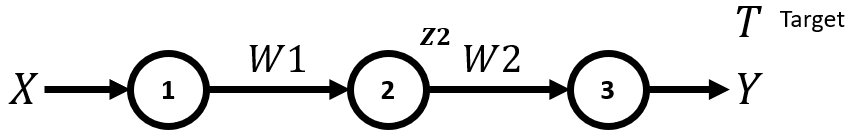
\includegraphics[scale=0.56]{Images/38.png} 
   \caption{Backpropagation}
\end{figure}

In forward propagation, it was assumed that all the weights and biases term are already optimized. Backpropagation is the process by which the weights and biases are optimized. Backpropagation uses gradient descent approach on each and every weight and bias term of the neural network. Since backpropagation is part of the training phase, it is performed on the training data $(X, T)$, where $X$ is the input and $T$ is the desired output or target. 
Here it is chosen the same simplistic neural network used in the forward propagation. For input $X$, if $Y$ is the output received for unoptimized weights. Here bias term are not considered for simplicity. 
The error is calculated as 
\[\text{Error} = (T - Y)^2\]
For optimizing the weight $W_1$, gradient descent approach is used
\[W_1=W_1-LR \cdot \frac{\partial Error}{\partial W_1}\]
Y is calculated as 
\[\text{Y}=\sigma(Z_2 \cdot W_2)=\sigma(\sigma(X \cdot W_1)\cdot W_2)\]
From gradient descent approach,
\[\frac{\partial Error}{\partial W_1}=\frac{\partial Error}{\partial Y} \cdot \frac{\partial Y}{\partial W_1}\]
\[\frac{\partial Error}{\partial W_1}=\frac{\partial Error}{\partial Y} \cdot (\frac{\partial Y}{\partial \sigma}\cdot \frac{\partial \sigma}{\partial Z_2} \cdot \frac{\partial Z_2}{\partial W_1})\]
The new $W_1$ is computed as
\[W_1=W_1-LR \cdot \frac{\partial Error}{\partial Y} \cdot (\frac{\partial Y}{\partial \sigma}\cdot \frac{\partial \sigma}{\partial Z_2} \cdot \frac{\partial Z_2}{\partial W_1})\]
The same process is repeated for all other weight and biases term in the neural network, for many number of time, until the minimum possible error is reached.
\section{Character recognition system using neural network}
A character recognition neural network model was implemented in MATLAB. Here the input was a 35-bit word suggesting a noisy alphabet. Moreover, the expected output from the system is a 26-bit word suggesting the original character.\\
The 35-bit noisy input can be represented in a 7 x 5 block or pixel, where each pixel can take a value of either 0 or 1. Pixels with value 1 are represented in black, and those with value 0 are represented in white.\\
For example, the character 'A' can be represented as\\ 
A: 01110 10001 10001 11111 10001 10001 10001\\
If some pixels are altered, it is a noisy version of the character. In this model, the noises can vary from 4-bit flips to 7-bit flips.\\
The 26-bit output is mapped to the 26 alphabet characters of the English language.\\
A: 1000000000000 0000000000000\\
B: 0100000000000 0000000000000\\
and so on\\
Z: 0000000000000 0000000000001\\
The model is trained on the original non-noisy character 35-bit word. After the training, the model should be able to predict the original character even when a noisy character is given as input.
\subsection{Neural architecture}
The neural architecture of the model can be obtained by continually adding hidden layers and hidden neurons and measuring the error, which uses the concept of overfitting and underfitting. If the hidden layer has very few neurons or very few numbers, it will lead to the condition underfitting. In such cases, the input is too complex to be handled by that many few neurons. However, if the number of hidden neurons and hidden layers is very high, the model is overly complex for the given input. The condition is known as overfitting.\\ 
In the case of overfitting, the model performs very well on the training data, and the error becomes approximately zero. However, it fails to generalize the input feature, and the error becomes very high for data other than training data (testing data).\\ 
In the case of underfitting, the model performs very poorly for both training data and testing data. 
So to find the optimum number of hidden layer neurons and hidden layer, the model should not overfit or underfit. The training error (error while working on the training data) and testing error (error while working on the testing data) are calculated. These errors are plotted against the number of neurons. That neuron is considered where the training and testing errors are close to each other.
\begin{figure}[H]
	\centering
   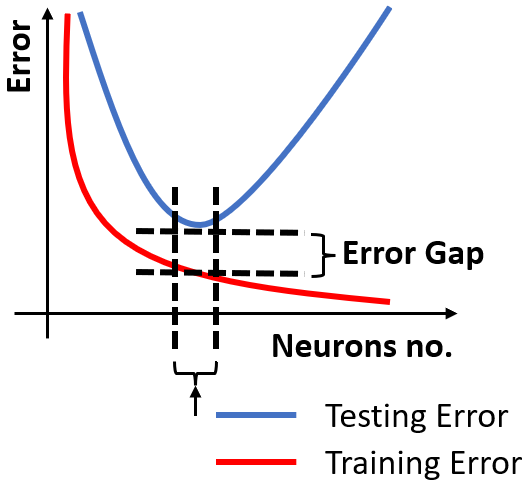
\includegraphics[scale=0.56]{Images/39.png} 
   \caption{Setting neural architecture}
\end{figure}



\section{Neural Network using Spintronics}
An electron along with a charge also contains spin. This spins can be used to store and transmit binary information, the UP spin encoded as 0 and DOWN spin as 1. Spintronic devices are rapidly developing nano technologies, they can store, process and communicate. It is just a matter of spin rotation, since no charge movement, hence there is no ohmic dissipation, but there prevails the dissipation due to magnetization damping. In order to change the spin,an external charge voltage/current is applied which inturn dissipates energy. At 100 nm dimension, all the spins align in one direction, which can be represented as one single large spin.~\cite{nature_news_art,roy15_1}\\
Multiferroics have gotten a lot of attention in recent days for devising energy-efficient devices~\cite{roy2020energy}~\cite{roy2017spintronics}. Recently, it has been shown that there can be a high-gain region in the input-output characteristics of the nanomagnets, which can harness the activation function for a neuron~\cite{roy2017ultralow}. Spintronic devices encapsulate the weight, sum, and activation function, which are the computing elements of the artificial neurons. Spintronic devices are non-volatile in nature, which saves us from adding extra circuitry to keep the data intact. Spintronic devices have long endurance, unlike transistor-based devices, which is why such devices are deployed in cars, missions to Mars etc. It can bear cosmic radiation, and other harsh interstellar space environments as well.~\cite{roy15_2}~\cite{roy15_3}
\subsection{Magnetic Anisotropy}
Magnetic anisotropy refers different magnetization in different directions. The magnetization of a specimen depends on its shape. When a specimen of finite size is magnetized by an external magnetic field, the free poles which appear on its ends will produce a magnetic field directed opposite to the magnetization. This field is called the demagnetizing field. The intensity of the demagnetizing field $H_d$ is proportional to the magnetic free pole density and therefore to the magnetization
\[H_d=N_d\frac{I}{\mu_0}\]
where $N_d$ is the demagnetizing factor, which depends on the shape of the specimen.\\
In case of a sphere, because of it total symmetry, the demagnetization factor is same in all direction, hence there is no anisotropy.
In case of an ellipsoid,as it is not symmetric in all direction, anisotropy exists but because of its oval shape, it is difficult to fabricate on a planar wafer.
Which makes an elliptical cylinder a best choice as it has inplane shape anisotropy and because of its planar surface, it is easy to fabricate on a planar wafer. The energy is given by 
\[E=\frac{1}{2}\Omega M_s H_k sin^2 \theta \] 
Where $\Omega$ is the volume of the elliptical cylinder, $M_s$ is the saturation magnetization, and $H_k$ is the coercive field

\subsection{Magnetic Field along In-plane: Easy and Hard axis}
\begin{figure}[H]
	\centering
   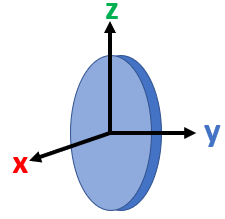
\includegraphics[scale=0.56]{Images/19.png} 
   \caption{Elliptical cylinder}
\end{figure} 
Switching magnetization from one direction to opposite direction by application of magnetic field in In-plane easy and hard axis. \\
In the Fig. 1.1, we have an elliptical cylinder whose major-axis is in the $\hat{z}$ direction, the minor-axis is in $\hat{y}$ direction and the thickness is in the $\hat{x}$ direction\\\\

\textbf{For In-plane hard axis}\\
\begin{figure}[H]
	\centering
   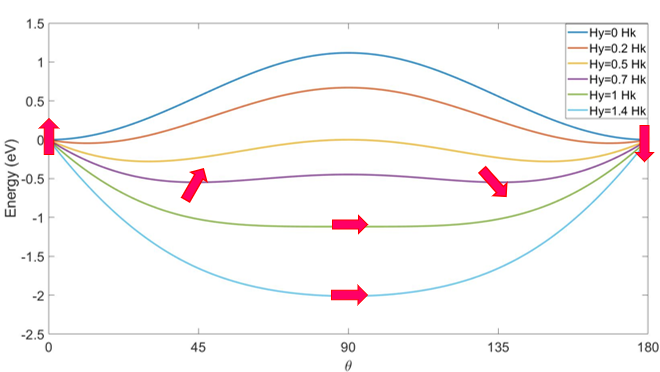
\includegraphics[scale=0.56]{Images/20.png} 
   \caption{In-plane hard axis: Energy vs $\theta$}
\end{figure}
The magnetic field (\textbf{$H_y$}) is applied along the $\hat{y}$ direction of the elliptical cylinder. The magnetization vector of the cylinder is making an angle $\theta$ with the z-axis. Let's assume, initially the magnetization vector is along the z-axis (i.z. $\theta=0^o$), on application of magnetic field $H_y$, can the magnetization vector be made align in (-z)-axis (i.z. $\theta=180^o$)

The anisotropic energy is given by 
\[E=\frac{1}{2}\mu_0M_sH_ksin^2\theta - \mu_0M_sH_ysin\theta\]
In Fig. 1.2, anisotropic energy is plotted against $\theta$($0^o - 180^o$) for different values of $H_y$.\\
For a given value of $H_y$, the magnetization vector aligns such that the anisotropic energy is minimum. Hence, \[\frac{dE}{d\theta}=0 \implies \theta_{min}=sin^{-1}(H_y/H_k)\]
The $\theta_{min}$ represent the angle made by the magnetization vector with the z-axis such that anisotropic energy is minimum. \\
When $H_y=0$, $\theta_{min}$ comes out to be $0^o$ ,and there is a potential barrier at $\theta=90^o$, which prevents the spontaneous magnetization flipping from $\theta=0^o$ to $180^o$. \\
As $H_y$ is increased gradually, the potential barrier at $\theta=90^o$ decreases and the $\theta_{min}$ shifts away from $\theta=0^o$, for example, when $H_y=0.7H_k$, $\theta_{min}=45^o$, i.z. on applying $H_y=0.7H_k$, the magnetization vector is making an angle of $45^o$ with the z-axis.\\\\
When $H_y=H_k$, $\theta_{min}=90^o$ and there is no potential barrier. But on further increasing the $H_y$ to however large value, the $\theta_{min}$ does not change, and it still remains at $\theta_{min}=90^o$.\\
Which suggest that on application of magnetic field along in-plane hard axis will not be able to switch the magnetization to the opposite direction.\\\\

\textbf{For In-plane easy axis}\\
\begin{figure}[H]
	\centering
   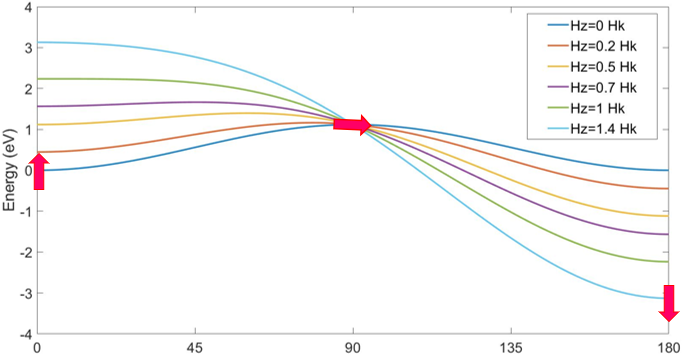
\includegraphics[scale=0.56]{Images/21.png} 
   \caption{In-plane easy axis: Energy vs $\theta$}
\end{figure}
When the magnetic field is applied along the $\hat{z}$ direction of the elliptical cylinder.The anisotropic energy is given by 
\[E=\frac{1}{2}\mu_0M_sH_ksin^2\theta - \mu_0M_sH_zcos\theta\]
For a given value of $H_z$, the magnetization vector aligns at an angle $\theta_{min}=sin^{-1}(H_z/H_k)$
In Fig. 1.3, anisotropic energy is plotted against $\theta$($0^o - 180^o$) for different values of $H_z$.
When $H_z=0$, $\theta_{min}$ comes out to be $0^o$ ,and there is a potential barrier at $\theta=90^o$, which prevents the magnetization flipping from $\theta=0^o$ to $180^o$. \\
On increasing the $H_z$, the energy at $\theta=0^o$ side increases and $\theta=180^o$ side decreases, thereby reducing the potential barrier.\\
When $H_z=H_k$, $\theta_{min}=90^o$ and instead of a potential barrier there is a potential down hill. So on further increasing the $\theta_{min}$ becomes $180^o$\\
Which concludes that when magnetic field is applied along the in-plane easy axis direction, magnetization switching is possible.  

\subsection{Perpendicular Magnetic Anisotropy}
\begin{figure}[H]
	\centering
  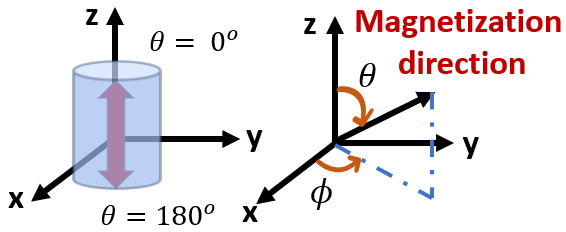
\includegraphics[scale=0.56]{Images/22.png}
  \caption{Perpendicular magnetic anisotropy}
\end{figure}
If the magnetization is in perpendicular direction to the planar surface, we have perpendicular magnetic anisotropy. For easy axis, $\theta = 0^o$ and $180^o$ and for the hard axis, $\theta = 90^o$.  The magnet's plane is $\phi=90^o$. Perpendicular magnetic anisotropy is essential as it decreases the lateral dimension, just like transistor scaling, it can accommodates more number of similar magnets in an area.~\cite{ikeda2010perpendicular}
\begin{figure}[H]
	\centering
  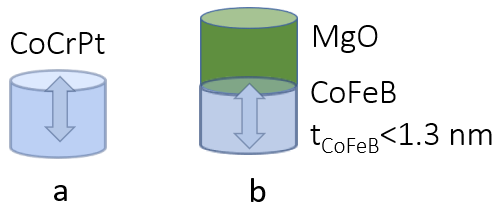
\includegraphics[scale=0.56]{Images/23.png}
  \caption{Perpendicular magnetic anisotropy: a. Bulk anisotropy b. Interface anisotropy}
\end{figure}
There are two type of perpendicular anisotropy: a. Bulk anisotropy and b. Interface anisotropy\\
\textbf{Bulk anisotropy:} \\
\textbf{Interface anisotropy:} This anisotropy occurred at the interface of two different material. It is seen that 	




\subsection{Magnetostriction}
Magnetostriction is a phenomenon where the shape of a ferromagnetic material changes during the process of magnetization. The deformation or the strain, $ \frac{\partial l}{l}$, generated is usually small and in the range $10^{-5}$ to $10^{-6}$.\\
On increasing the magnitude of magnetic field, the magnetostriction strain increases. After a certain magnetic field the strain reaches a saturation value $\lambda$ and known as the magnetostrictive co-efficient.
\begin{figure}[H]
	\centering
   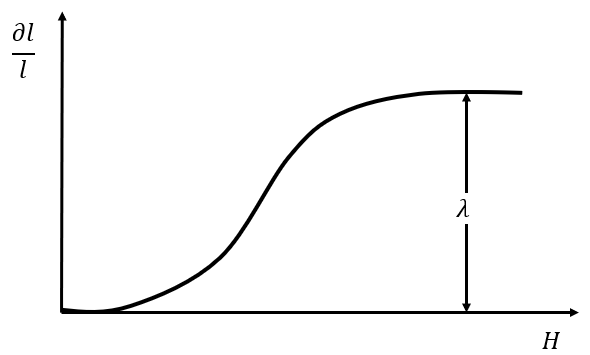
\includegraphics[scale=0.56]{Images/24.png} 
   \caption{Magnetostriction elongation vs applied field}
\end{figure}
The reason behind this phenomenon is the crystal structure inside the domain spontaneously deforms in the direction of magnetization and the strain axis rotates with the magnetization creating a deformation therby generating strain.\\
The spontaneous strain in the domain is expressed as $e=\frac{3}{2} \lambda$\\
The magnetostriction strain depends on the angle $\psi$, made by the applied magnetic field with the easy axis of the ferromagnetic specimen.
\[\Delta(\frac{\partial l}{l})=\frac{3}{2}\lambda(1-cos^2\psi)\]
The higher the magnetic field, the domain magnetization rotates more towards the direction of the applied field. If H is parallel to the easy axis $\Delta(\frac{\partial l}{l})=0$, that is there will be no elongation or no strain generated.
\subsection{Multiferroics and Multiferroic Composites}
\begin{figure}[H]
	\centering
   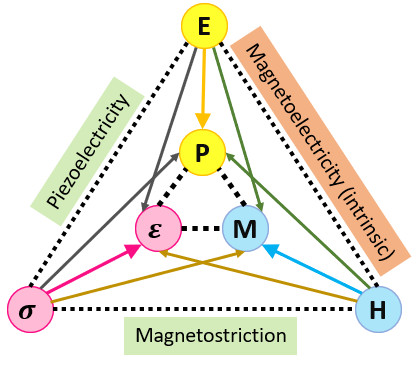
\includegraphics[scale=0.56]{Images/18.png} 
   \caption{Multiferroics}
\end{figure}
In nature there exist, ferroelectric and ferromagnetic materials. \\
\textbf{Ferroelectric materials} are those materials whose polarization changes on changing the electric field and vice versa.\\
Similar to ferroelectric, the \textbf{ferromagnetic materials} are those materials whose magnetization changes on changing the magnetic field and vice verse.~\cite{RefWorks:165} \\\\
There are certain materials which posses both the properties of ferroelectric and ferromagnetic materials. These materials are known as \textbf{multiferroics}. For a multiferroic material, the polarization changes on changing the magnetic field and the magnetization changes on changing the electric field.\\   
In the Figure 1.1, the outer node of the triangle which consists of Electric field \textbf{E}, Magnetic field \textbf{H}, and the Stress \textbf{$\sigma$} are the physical parameters which can be changed, and the inner node of the triangle which consists of Polarization \textbf{P}, Strain \textbf{$\epsilon$}, and the Magnetization \textbf{M} are the  macroscopic observables of the respective physical parameter.\cite{roy14_6}~\cite{RefWorks:164}\\
Ferroelectric material: change in E leads to change in P\\
Ferromagnetic material: change in H leads to change in M and\\
Ferroelastic material: change in $\sigma$ leads to change in $\epsilon$\\
For multiferroic material there is an intrinsic coupling between \textbf{E} and \textbf{H}, known as Magneto-electric coupling
\[\alpha_{ME}=\mu_0\frac{\partial M}{\partial E}\]
At room temperature the magneto-electric coupling is very weak. So instead of a multiferroics, a multiferroic composite is used~\cite{RefWorks:842}. Which is a composite of pizeoelectric and magnetostrictive material. Piezoelectric materials are those materials, on applying electric field, stress is generated at the body and vice versa, and magnetostrictive material are those materials which generates stress on application of magnetic field, and vice versa. The composition of piezoelectric and magnetostrictive material serves the same purpose of multiferroics with strong magneto-electric coupling. Multiferroic composites are stress mediated materials.~\cite{RefWorks:164}
\[\alpha_{ME}=\mu_0\frac{\partial M}{\partial \sigma}\frac{\partial \sigma}{\partial E}\] 

\subsection{Giant Magnetoresistance (GMR)}
\begin{figure}[H]
	\centering
   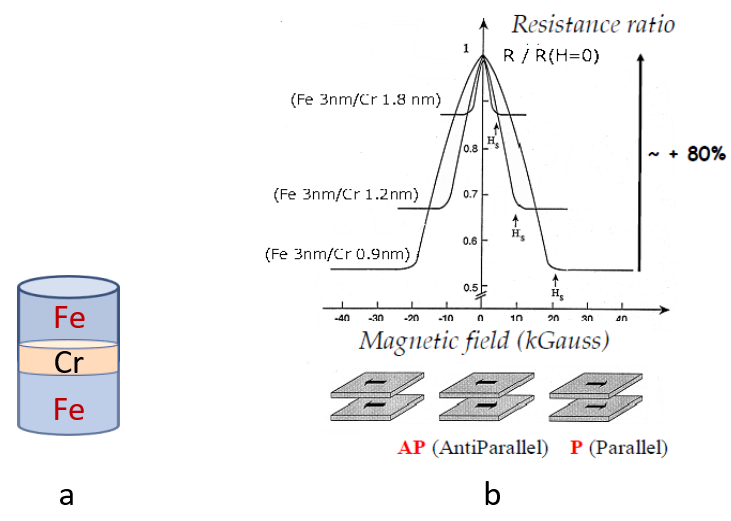
\includegraphics[scale=0.56]{Images/25.png} 
   \caption{Giant Magneto Resistance}
\end{figure}
In 2007, Nobel prize in physics was awarded jointly to Albert Fert and Peter Grunberg, for the discovery of Giant magnetic resistance~\cite{baibich1988giant}~\cite{binasch1989enhanced}. In the Figure 1.8(a), there is a structure Fe/Cr/Fe, it is seen that on application of magnetic field the resistance along the structure reduces. In Figure 1.8(b), the resistance ratio vs Magnetic field is plotted against three different thickness of  the chromium layer.\\
The origin of the phenomenon is that the magnetization of the Fe layers in the either side of the Cr layer are in anti-parallel orientation as a result of negative exchange interaction through the Cr layer. On application of magnetic field, the spin-dependent magnetic scattering of conduction electron is reduced, which causes a parallel orientation.\\
The GMR is calculated as follows
\[GMR=\frac{R(0)-R(H)}{R(H)}\]
where $R(0)$ refers to resistance when no magnetic field is applied, $R(H)$ refers to resistance when magnetic field is applied.
\subsection{Tunnelling Magnetoresistance (TMR)}
\begin{figure}[H]
	\centering
   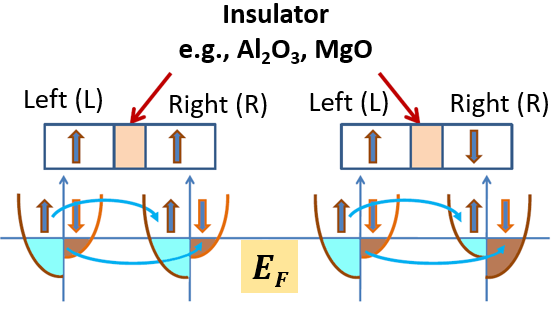
\includegraphics[scale=0.56]{Images/26.png} 
   \caption{Tunnelling Magneto Resistance}
\end{figure}
Magnetic tunnelling is observed for two ferromagnetic metal layers separated by a thin insulating materials like $Al_2O_3$, $MgO$~\cite{julliere1975tunneling}. Similar to GMR, in case of TMR, when the magnetization on both the ferromagnetic layers are in parallel orientation, resistance is low and when they are in anti-parallel orientation, the resistance is high~\cite{moodera1995large}~\cite{miwa2014highly}.\\
This phenomenon occurs because below the fermi level, for a UP magnetization, the density of UP states is higher than the density of DOWN states.Similarly, for DOWN magnetization, the density of the DOWN state is higher than the density of UP state.~\cite{RefWorks:786}\\
So for parallel orientation as shown in the Figure 1.9, for both side of the insulator, below the fermi level, the density of UP state is equal on both side ($N_L^{\uparrow}=N_R^{\uparrow}$), similar is the case for DOWN state ($N_L^{\downarrow}=N_R^{\downarrow}$). Hence, the states or the electrons can easily tunnel, and results in low resistance. But in case of anti-parallel orientation, the respective density of states are not same on the both side. In Figure 1.9, for the anti-parallel case, the density of UP state is high in the left side while the density of UP state in the left side low ($N_L^{\uparrow}>N_R^{\uparrow}$). Hence the electrons can not easily tunnel through the insulator, and results in increasing resistance.~\cite{RefWorks:300}~\cite{RefWorks:33}\\
The conductance is proportional to density of states:$N_L^{\uparrow},N_R^{\uparrow},N_L^{\downarrow},N_R^{\downarrow}$\\
\[TMR=\frac{G_P-G_{AP}}{G_{AP}}\]
Where $G_P=G^{\uparrow \uparrow}+G^{\downarrow \downarrow}$ and $G_{AP}=G^{\downarrow \uparrow}+G^{\uparrow \downarrow}$, and the conducatance are proportional to the density of states.\\
$G^{\uparrow \uparrow} \propto N_L^{\uparrow}N_R^{\uparrow}$,\\
$G^{\downarrow \downarrow} \propto N_L^{\downarrow}N_R^{\downarrow}$,\\
$G^{\downarrow \uparrow} \propto N_L^{\downarrow}N_R^{\uparrow}$, and\\
$G^{\uparrow \downarrow} \propto N_L^{\uparrow}N_R^{\downarrow}$
\section{Magnetic Thermal Annealing}
Lattice and shape deformities in a material can significantly degrades its quality. Thermal annealing is a common technique used to strengthen the solid by raising, maintaining, and slowly decreasing the temperature. Raising the temperature allows the atoms to diffuse more easily to their proper location, and maintaing the temperature attains equilibrium, eliminating any structural imperfections.\\
When magnetic field is applied during the thermal annealing process, it is known as Magnetic thermal annealing. It has some interesting effect in ferromagnetic materials. The most important one is the re-orientation of the easy axis of a magnetic material. In any magnetic material, the easy axis is determined by the lattice structure of the material. If the shape shows any symmetry , the easy axis will normally reflect this symmetry. Now if there are many structural deformities , then there would be no global symmetry and the easy axis will be randomized.\\
When a deformed ferromagnetic material is thermally annealed in presence of an externally applied magnetic field, the spins of each individual atom will align the direction of the applied magnetic field. When maintained at high temperature, the system will attain equilibrium within this field, causing a lattice re-orientation such that easy axis is parallel to the applied magnetic field.
\subsection{Magnetic Thermal Annealing experimental system}
\begin{figure}[H]
%\begin{subfigure}
	\centering
   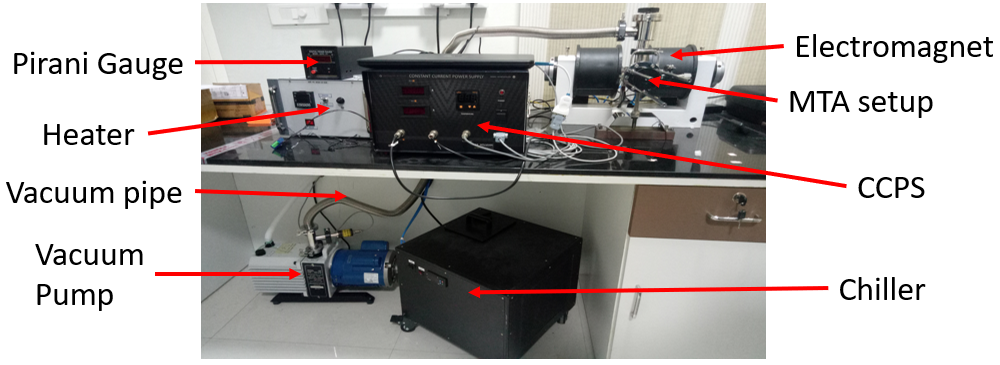
\includegraphics[scale=0.56]{Images/27.png} 
   \caption{Magnetic Thermal Annealing experimental system}
   %\end{subfigure}
\end{figure}
In Figure 1.10, the experimental set-up for magnetic thermal annealing is shown. Where there is an electromagnet which provides constant DC magnetic field, there is a Constant Current Power Supply (CCPS) to provide constant current to the electromagnet, there is a chiller, to liquid cool the coils of the electromagnet, then there is the annealing set-up, inside which sample is placed. Inside the annealing set-up, there is a thermocouple, which generates heat. The thermocouple is connected to the heater PID which controls the amount and the duration of heating. The magnetic thermal annealing is done in vacuum, for which there is a rotatory vacuum pump connected to the annealing set-up. To monitor the vacuum pump pressure, a pirani gauge is connected to the vacuum pump.    
\section{Ferro-magnteic Resonance (FMR)}
When a magnetic material is placed in a DC magnetic field, the magnetization vector rotates in counter-clock wise direction, along the direction of the DC field. This is called the precessional motion of the magnetization vector, as it does, it losses energy, the rotational body falls in the direction of the DC field, this is known as damping. This precesssing of magnetization vector is captured by the   Landau-Lifshitz Equation (LL Equation):
\[\frac{dM}{dt}=-|\gamma|M\times H_{eff} - \frac{\alpha |\gamma|}{M}M\times M\times H_{eff}\]
where $\alpha$ and $\gamma$ are the damping parameter and the Gyromagnetic ratio of the magnetic material respectively.\\
In FMR experiment our aim is to find $\alpha$ of the magnetic material.\\
We will consider $\alpha$ later. The precessional motion of the magnetization vector is given by 
\[\frac{dM}{dt}=-|\gamma|M\times H_{eff}\]
DC magnetic field is applied along the z-axis, hence $M_z=M$, and the $M_x$ and $M_y$ has $e^{-i\omega t}$ dependence, hence
\[\frac{dM_x}{dt}=-|\gamma|(H_z + (N_{yy}-N_{zz})M)M_y\]
and
\[\frac{dM_y}{dt}=|\gamma|(H_z + (N_{xx}-N_{zz})M)M_x\]
Solving the above two equation, we get
\[\omega^2=|\gamma|^2(H_z + (N_{yy}-N_{zz})M)(H_z+(N_{xx}-N_{zz})M)\]
In case of, sphere: $N_{xx}=N_{yy}=N_{zz}$, therefore, $\omega =|\gamma|H_z$\\
In-plane FMR: $N_{xx}=N_{zz}=0, N_{yy}=1$, therefore, $\omega =|\gamma|\sqrt{H_z(H_z+M)}$\\
Perpendicular FMR:  $N_{xx}=N_{yy}=0, N_{zz}=1$, therefore, $\omega =|\gamma|(Hz-M)$\\
On Linearizing the small rotations,
\[\frac{d^2\phi}{dt^2}+\alpha|\gamma|M\frac{d\phi}{dt}+\omega_0^2\phi=0\]
where $\omega_0=|\gamma|\sqrt{H_z(H_z+M)}$, for IN-plane FMR\\
To negative the damping, and to keep the magnetization rotating, a transverse AC field $H_y(t)=H_{y0}e^{i\omega t}$ is applied
\[\frac{d^2\phi}{dt^2}+\alpha|\gamma|M\frac{d\phi}{dt}+\omega_0^2\phi =|\omega|^2MH_{y0}e^{i\omega t} \]
On solving the differential equation, $\phi(t)=\phi_0e^{i\omega t}=|\phi_0|e^{i(\omega t+\delta)}$, where\\
\[\phi_0=\frac{|\gamma|^2MH_{y0}}{(\omega_0^2 - \omega^2)^2 + (\alpha|\gamma|M\omega)^2}[(\omega_0^2 - \omega^2)-i\alpha|\gamma|M\omega]\]
\[|\phi_0|=\frac{|\gamma|^2MH_{y0}}{\sqrt{(\omega_0^2 - \omega^2)^2 + (\alpha|\gamma|M\omega)^2}}, tan \delta = \frac{-\alpha|\gamma|M\omega}{(\omega_0^2 - \omega^2)}\]
The FMR absorption is given by the Imag($\phi_0$), known as the Lorentzian
\[Imag(\phi_0)=\frac{|\gamma|^2MH_{y0}\alpha|\gamma|M\omega}{(\omega_0^2 - \omega^2)^2 + (\alpha|\gamma|M\omega)^2}\]
at $\omega=\omega_0$, $Imag(\phi_0)=\frac {H_{y0}|\gamma|}{\alpha \omega_0}$\\
The FMR linewidth $\Delta H$, Half width at half maximum (HWHM) is given by:
\[\Delta H =\frac{\alpha\omega_0}{|\gamma|}\]

%\chapter{Method} \label{ch: method}
\section{Electron Beam Lithography}
Electron beam (e-beam) lithography is a method that utilizes an electron gun from a scanning electron microscope. This method is used to draw patterns at nano-meter levels. In which the electrons are exposed to a film of photoresist, which reacts with the electrons. Generally, there are two types of photoresists, namely positive photoresists and negative photoresists. When a positive photoresist is exposed to the electron beam, those part which is exposed to the electron beam becomes soluble to the photoresist developer solution. But when a negative photoresist is exposed to the electron beam, those parts that are exposed become hard and the rest part becomes soluble to the photoresist developer solution.
\subsection{Procedure}
\begin{itemize}
	\item At first the wafer is cleaned inside ultrasonic cleaner 3 times with electronic grade acetone and 1 time with methanol
	\item Which then cleaned with DI water, to remove any remains of acetone or methanol
	\item Then the wafer is cleaned and dried by blowing Nitrogen gun
	\item After which the wafer is dehydrated to remove moisture using a hot plate
	\item Then the wafer is kept on the spin coater chuck, and adequate amount of photoresist is drooped on the wafer, and is rotated at certain RPM to get the required thickness
	\item Once spin coating is done, the wafer is pre-baked by putting on hot plate, so that photoresist become hard
	\item Then electron beam is exposed to the photoresist area
	\item Then the exposed sample is placed inside the developer solution (IPA:MIBK=3:1 + 2\% DI water)
	\item After which sputtering is performed
	\item Then lift off process is done to remove the photoresist layer 
	
\end{itemize}    
\section{Magnetic Force Microscopy (MFM)}
\begin{figure}[H]
%\begin{subfigure}
	\centering
   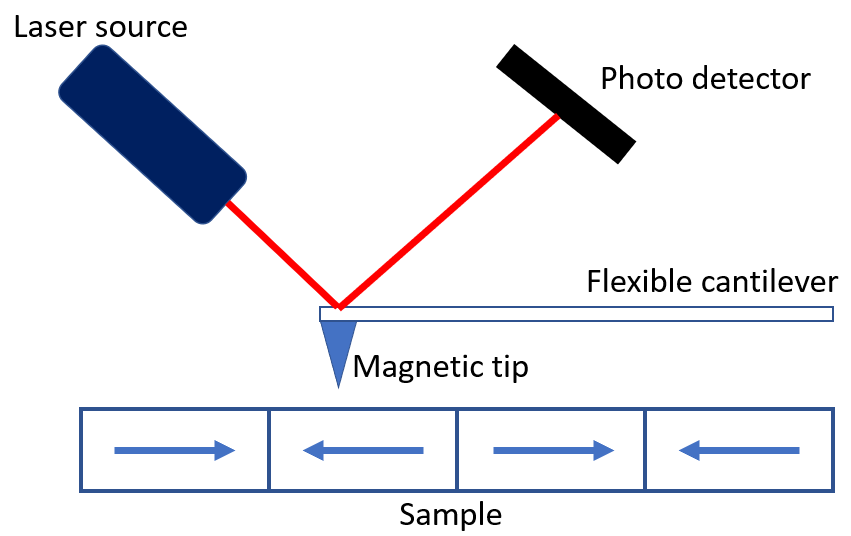
\includegraphics[height=6cm]{Images/53.png} 
   \caption{Magnetic Force Microscopy (MFM)}
   %\end{subfigure}
\end{figure}
Magnetic force microscopy or MFM is used for imaging the magnetic domains of a magnetic sample.
It consists of a flexible cantilever, a magnetic tip on the front of the cantilever, and then a laser aligned to the top of the cantilever. There is a photo detector that detects the reflected laser from the cantilever. The tip is scanned over the magnetic sample. Since the tip is magnetized, it is either attracted or repelled from the sample based on the magnetization direction of each domain. Based on the force acting on the tip, the cantilever moves up and down, deflecting the laser received at the photo detector. Based on the degree of deflection, the imaging of the sample is done.
\section{Vibrating Sample Magnetometer (VSM)}
\begin{figure}[H]
%\begin{subfigure}
	\centering
   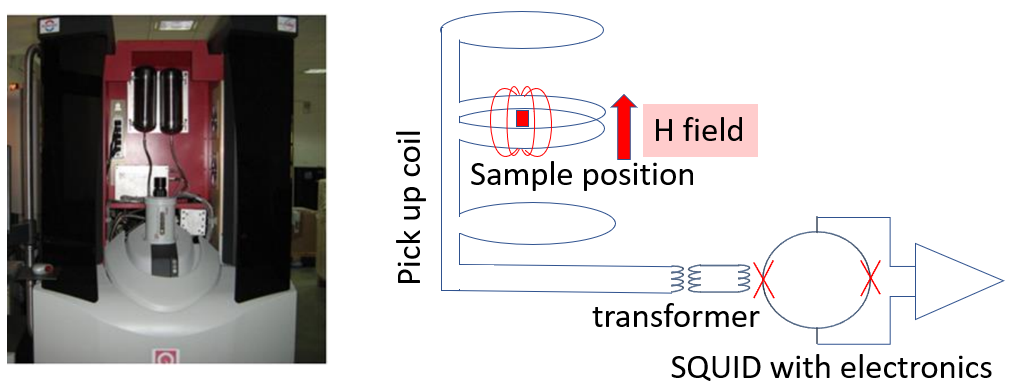
\includegraphics[width=12cm]{Images/54.png} 
   \caption{Vibrating Sample Magnetometer (VSM)}
   %\end{subfigure}
\end{figure}
Vibrating sample magnetometer or VSM is a highly sensitive instrument used for precise magnetic moment measurements. It operates on the basic principle of Faraday's law. It is useful in measuring the magnetic behavior of a magnetic material.\\
The instrument consists of an electromagnet, which generates a constant DC magnetic field. There is a driver rod over which the magnetic sample is pasted. The rod can oscillate in the vertical direction with some fixed frequency and amplitude. When the sample is brought into the DC field, the constant magnetic field magnetizes the sample, and the magnetization vector aligns in the direction of the DC field. Due to this, the samples create it's own magnetic field when the driver rod starts oscillating—the magnetic field due to the sample changes with respect to the time. There are pick-up coils beside the sample, which pick up the alternating magnetic field and generates an electric field in the pick-up coil based on Faraday's law. The induced current is then amplified and sent to the Superconducting Quantum Interference Device (SQUID).
%\section{X-ray Diffraction (XRD)}
\section{X-ray Reflectivity (XRR)}
X-ray reflectivity, or XRR, is a measurement technique that uses X-ray reflection intensity to determine the thickness of a multilayer thin-film structure. 
When an x-ray beam falls on the surface of a layer, if the incident angle, $\theta_i<\theta_c$, where $\theta_c$ is the critical angle, total reflection occurs, if $\theta_i=\theta_c$ the beam propagates along with the layer, and if $\theta_i>\theta_c$ some part of the reflects and refracts.\\\\ 
The X-ray intensity curve is plotted between the intensity of the reflected x-ray and the incident angle. When an x-ray beam falls on the surface of the layers, some part of the beam is reflected, and some part gets refracted. The observed x-ray scattering is the sum of individual electron scattering. When the reflected ray hits another layer, it is either totally reflected or reflected and refracted. This reflected ray from the interface of $1^{st}$ and $2^{nd}$ medium interfere with each other, which gives rise to oscillation. This oscillation depends on the film thickness; the thicker the film, the shorter the oscillation time period.  
\section{Experimental Apparatus}
This list of experimental apparatus used in the entire project is mentioned here
\subsection{Spin Coater}
\begin{figure}[H]
%\begin{subfigure}
	\centering
   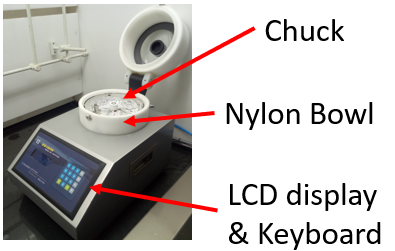
\includegraphics[scale=0.56]{Images/4.png} 
   \caption{Spin Coater}
   %\end{subfigure}
\end{figure}
For spin-coating EBL photo-resist of 100 nm thickness on a Si substrate a Holmarc Spin-coater is used. It has a nylon bowl, inside which there is a chuck which holds the sample using a vacuum pump. In the front-panel, there is a LCD display and keyboard to program the Spin-coaters rotation speed, acceleration, time period of rotation, and number of steps.

\subsection{Shaker}
\begin{figure}[H]
%\begin{subfigure}
	\centering
   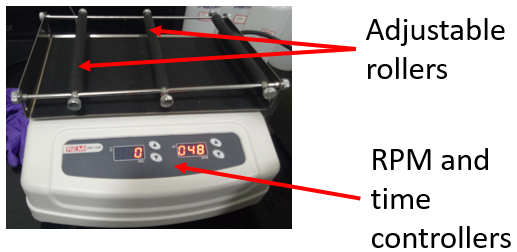
\includegraphics[scale=0.56]{Images/5.png} 
   \caption{Shaker}
   %\end{subfigure}
\end{figure}
To shake or mixing chemicals, the shaker is used. It has adjustable rollers which helps in fixing the beaker firmly on the movable platform. On the front-panel there are buttons to set the RPM and the time duration.

\subsection{Hot Plate}
\begin{figure}[H]
%\begin{subfigure}
	\centering
   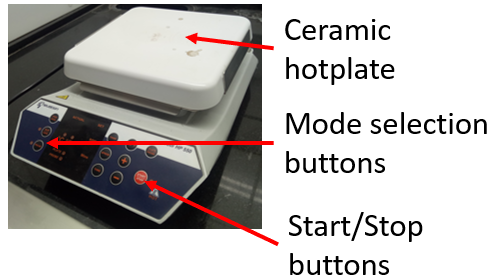
\includegraphics[scale=0.56]{Images/6.png} 
   \caption{Hot plate}
   %\end{subfigure}
\end{figure}
To bake samples at high temperature, a hot plate is used. It has a ceramic platform, over which samples are placed. The ceramic plate can go up to $550^o C$. In the front-panel there buttons to set the temperature, timer and start/stop button.

\subsection{Ultrasonic Cleaner}
\begin{figure}[H]
%\begin{subfigure}
	\centering
   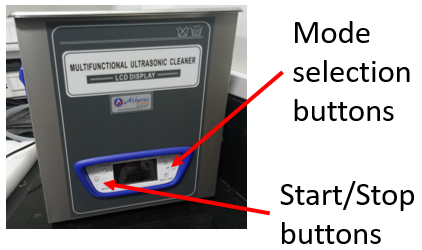
\includegraphics[scale=0.56]{Images/7.png} 
   \caption{Ultrasonic cleaner}
   %\end{subfigure}
\end{figure}
To clean samples, beakers or other apparatus by vibrating at high frequency. Samples are placed inside a cleaner, with appropriate solvent which gets cleaned on vibrating. In the front-panel there are buttons for Start/Stop, timer, temperature.

\subsection{Hot Air Oven}
\begin{figure}[H]
%\begin{subfigure}
	\centering
   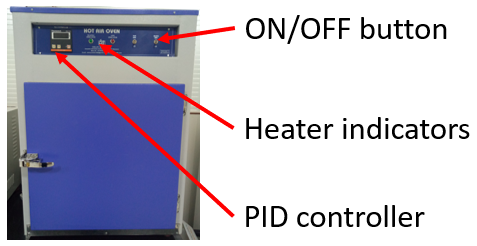
\includegraphics[scale=0.56]{Images/8.png} 
   \caption{Hot air oven}
   %\end{subfigure}
\end{figure}

To sterilize the samples using dry air, a hot air oven is used. Inside there is a thermostat to control the temperature. The inside wall are thermally insulated, hence it keeps the heat inside. On the front panel, it has ON/OFF button, an heater indicator to indicate the heating status, and there is a PID controller, which controls the thermostat.  

\subsection{Rota Mantle}

\begin{figure}[H]
%\begin{subfigure}
	\centering
   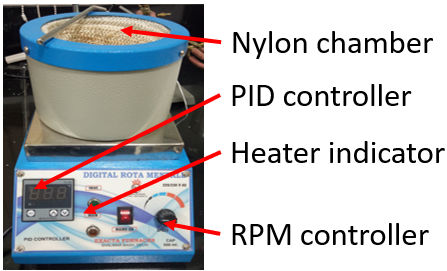
\includegraphics[scale=0.56]{Images/9.png} 
   \caption{Rota Mantle}
   %\end{subfigure}
\end{figure}
To heat up solvents while stirring with help of a magnetic bead. Usually used in the distillation process of chemicals. It has nylon chamber inside which the glass apparatus like round-bottom flask is placed. On the front panel, there is a PID controller, which programs the heating. Then there is a heater indicator, which displays the heating status and there is a RPM controller, which controls the RPM of the magnetic bead used while stirring. 

\subsection{Nitrogrn Gun}
\begin{figure}[H]
%\begin{subfigure}
	\centering
   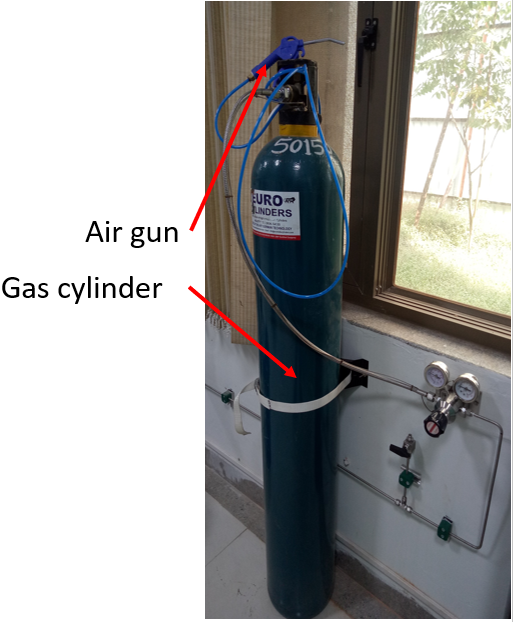
\includegraphics[height=5cm]{Images/10.png} 
   \caption{Nitrogen Gun}
   %\end{subfigure}
\end{figure}
To clean wafers by blowing $N_2$ gas. There is pipe all over the lab which connects to a $N_2$ cylinder, and there is outlets at work stations, where an air gun can be used to blow directly on the wafers.

\subsection{Vacuum Desiccator}
\begin{figure}[H]
%\begin{subfigure}
	\centering
   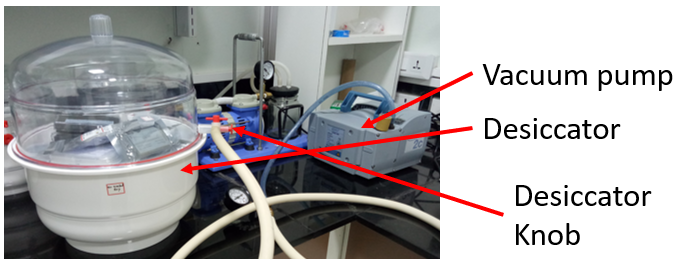
\includegraphics[scale=0.56]{Images/11.png} 
   \caption{Vacuum Desiccator}
   %\end{subfigure}
\end{figure}
To keep samples in vacuum which are prone to outside environment such as oxygen, moisture etc. The samples are placed inside the desiccator, and the lid is closed. A vacuum pump is connected to the desiccator knob, and the inside of the desiccator is made vacuum. After that the knob is closed.

\subsection{Muffle Furnace}
\begin{figure}[H]
%\begin{subfigure}
	\centering
   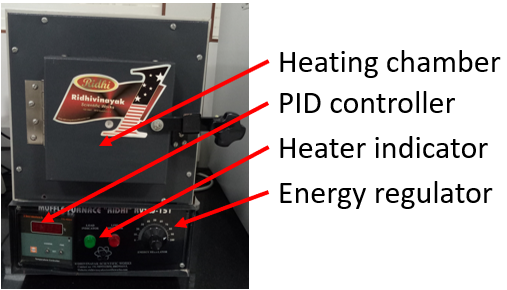
\includegraphics[scale=0.56]{Images/12.png} 
   \caption{Muffle furnace}
   %\end{subfigure}
\end{figure}
To thermally anneal samples at higher temperature to passivate all dangling bond and structural imperfection. The muffle furnace can reach upto $1200^oC$. In the front panel, there is a PID controller, which program and regulated the heating of the furnace. There is a heating indicator, to indicate the heating status of the device. There is a energy regulator, to control the power of the furnace. The samples as placed inside the heating chamber, which has insulated inner walls to prevent the heat loss.  

\subsection{Fume Hood}
\begin{figure}[H]
%\begin{subfigure}
	\centering
   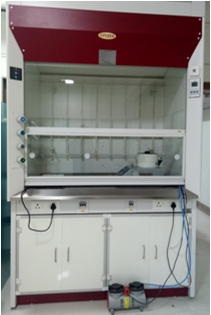
\includegraphics[scale=0.56]{Images/13.png} 
   \caption{Fume hood}
   %\end{subfigure}
\end{figure}
To carry out all chemical related experiment, which can eject harmful fumes. It can prevent from accidental spillage of harmful chemicals. Inside there are nozzles for different gas like $N_2$, $O_2$, etc. 

\subsection{Source Measuring Unit (SMU)}
\begin{figure}[H]
%\begin{subfigure}
	\centering
   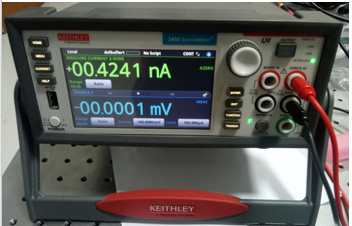
\includegraphics[scale=0.56]{Images/14.png} 
   \caption{Source Measuring Unit (SMU)}
   %\end{subfigure}
\end{figure}
Source Measuring Unit or SMU is a four-quadrant device; it can both source and measure simultaneously. It is a very high precision device and has high tolerance toward noise. It can also be used as a constant current source and also used for resistance measurement.


\subsection{Power Supply}
\begin{figure}[H]
%\begin{subfigure}
	\centering
   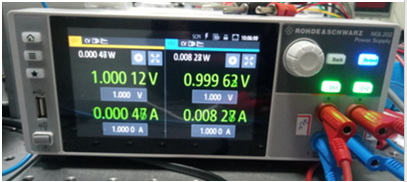
\includegraphics[scale=0.56]{Images/15.png} 
   \caption{Power Supply}
   %\end{subfigure}
\end{figure}
A power supply is a two-quadrant device; it can only act as a source. It is used as a DC voltage source. It is a two-independent channel that can be used to source DC voltage.  

\subsection{Probe Station}
\begin{figure}[H]
%\begin{subfigure}
	\centering
   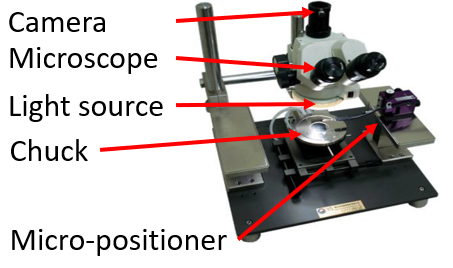
\includegraphics[scale=0.56]{Images/16.png} 
   \caption{Probe Station}
   %\end{subfigure}
\end{figure}
A probe station is used for the electrical measurement of samples with a smaller dimension which cannot be done with regular probes. The device consists of a chuck on top of which the samples are placed. Conclusion: there is a microscope and light source that enables visualization of the sample while making contacts. For making contacts, micropositioners are used, whose tips can be as small as 1um in diameter. The micropositioner can be connected to a power supply to apply the stimulus.

\subsection{Oscilloscope}
\begin{figure}[H]
%\begin{subfigure}
	\centering
   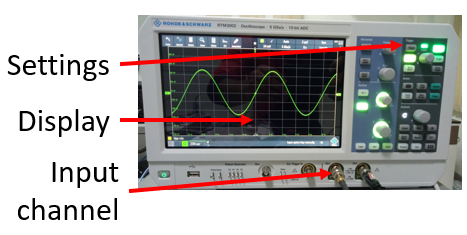
\includegraphics[scale=0.56]{Images/17.png} 
   \caption{Oscilloscope}
   %\end{subfigure}
\end{figure}
An oscilloscope is used for visualizing electrical signals and how they change over time. It is generally used to measure the AC voltage in circuits. It can do the Fourier analysis on any time-varying signal. The frequency range of the oscilloscope is 0.01 Hz to 100 MHz.

\chapter{Results} \label{ch: results}

\section{Character recognition system using neural network}
\subsection{Neural architecture modeling}
For the character recognition system, initially, the model was given one hidden layer, and the number of hidden layer neurons was increased from 1 to 200. The respective error vs. no. of neurons was plotted. It is seen that after 40 neurons, the error gap started increasing. Therefore the first hidden layer has 40 hidden neurons. Now the model was given two hidden layers. The first hidden layer has 40 neurons, and the second hidden layer's neurons vary from 1 to 200. It is seen that the error gap started increasing after the 35th neuron. However, the error gap of the model with the two hidden layer systems was more than the single hidden layer system, which suggested that the model is overfitting. So to make sure, another hidden layer was added, and the same procedure was followed, the error gap increased even further. Hence the optimized number of hidden layers and hidden layer neurons is one hidden layer with 40 hidden neurons.
\[[35\text{ input nodes}] \longrightarrow [40\text{ hidden nodes}] \longrightarrow [26\text{ output nodes}]\] 

\begin{figure}[H]
	\centering
   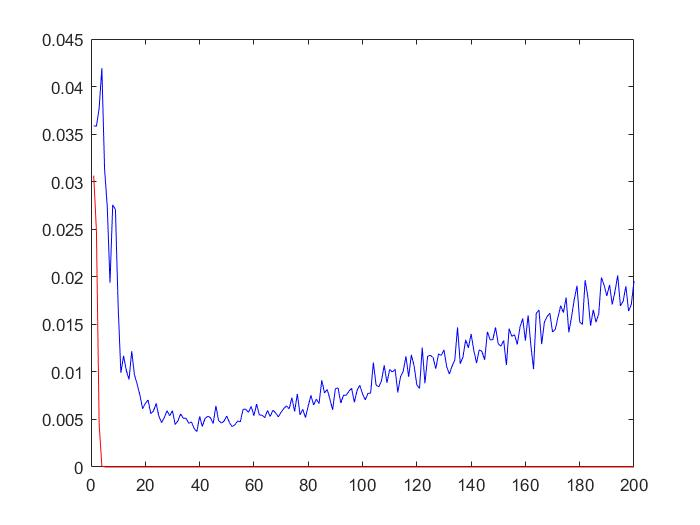
\includegraphics[height=7.1cm]{Images/40.png} 
   \caption{Optimizing first hidden layer}
\end{figure}
\begin{figure}[H]
	\centering
   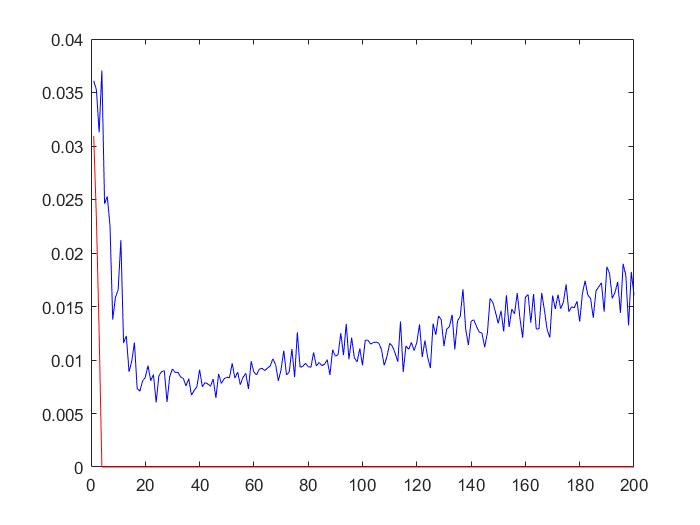
\includegraphics[height=7.1cm]{Images/41.png} 
   \caption{Optimizing second hidden layer}
\end{figure}
\begin{figure}[H]
	\centering
   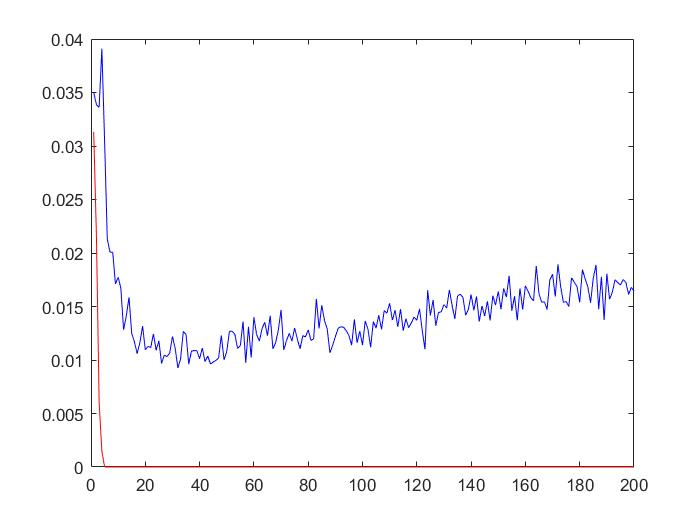
\includegraphics[height=7.1cm]{Images/42.png} 
   \caption{Optimizing third hidden layer}
\end{figure}
\subsection{Model output}
The model was trained on 26 data depicting the original non-perturbed data, and the testing of the model was done on data with different degree of perturbation.\\\\
\begin{minipage}{0.5\linewidth}
\textbf{For 4-bit flip}\\
Testing data: 520\\
No. of correct predictions: 424\\
No. of wrong predictions: 96\\
Accuracy of the model: 81.54\%   \\
\end{minipage}
\hfill
\begin{minipage}{0.6\linewidth}
\textbf{For 6-bit flip}\\
Testing data: 520\\
No. of correct predictions: 365\\
No. of wrong predictions: 155\\
Accuracy of the model: 70.19\%   \\
\end{minipage}
\begin{minipage}{0.6\linewidth}
\textbf{For (4 to 8)-bit flip}\\
Testing data: 2678\\
No. of correct predictions: 1866\\
No. of wrong predictions: 812\\
Accuracy of the model: 69.68\%   \\
\end{minipage}

  
\section{Improvement of magnetization using Magnetic Thermal Annealing (MTA)}
To test the improvement of magnetization using magnetic thermal annealing. A magnetic sample was take, from substrate side Ta(5)/MgO(0.8)/CoFeB(10). All the numbers inside the bracket are the nominal thickness of the material deposited in nano-meter. This sample was processed through magnetic thermal annealing along the In-plane easy axis direction. The magnetic thermal annealing was done at $400$ mT magnetic field, maintained at $400^oC$ for 1 hour at $10^{-3}$ Torr in vacuum. The experimental VSM results of the sample before (in blue) and after (in red) the MTA is shown in the following figure.
\begin{figure}[H]
	\centering
   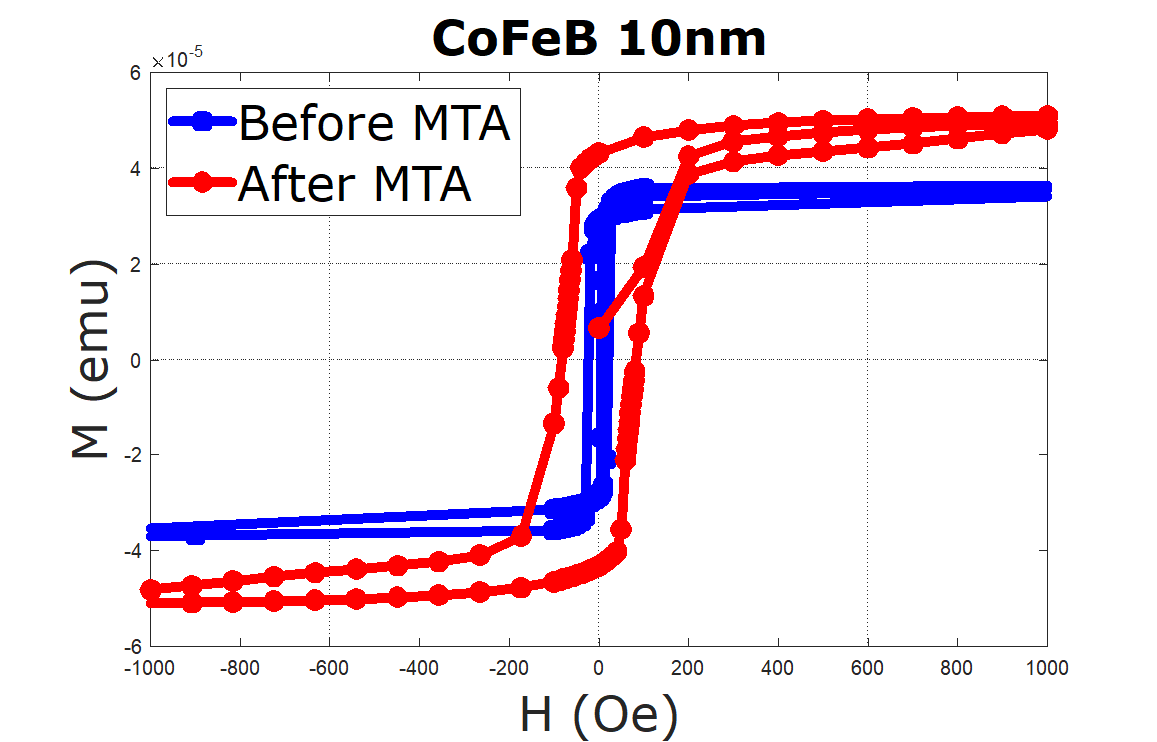
\includegraphics[height=7.1cm]{Images/37.png} 
   \caption{MTA of CoFeB 10nm sample}
\end{figure}
From the blue curve, it is seen that before MTA the CoFeB sample, has a coercive field, $H_k$ = 21 Oe and Magnetization, M = $3.7\times10^{-5}$ emu.\\
\\
From the red curve, it is seen that after MTA, the CoFeB sample, has $H_k$ = 70 Oe and M=$5.2 \times 10^{-5}$ emu.\\
After MTA there is a 18.5 times more M-H area. Which suggest that upon doing magnetic thermal annealing, there is improvement in the magnetization of the CoFeB 10nm sample.

\section{Development of LabView environment for different instruments}
\subsection{Power supply} 
To automate the power supply and for data acquisition, LabVIEW was used. The two-channel power supply was automated to obtain the VI curve of a resistor and a diode and the input characteristics of a transistor.
\begin{figure}[H]
%\begin{subfigure}
	\centering
   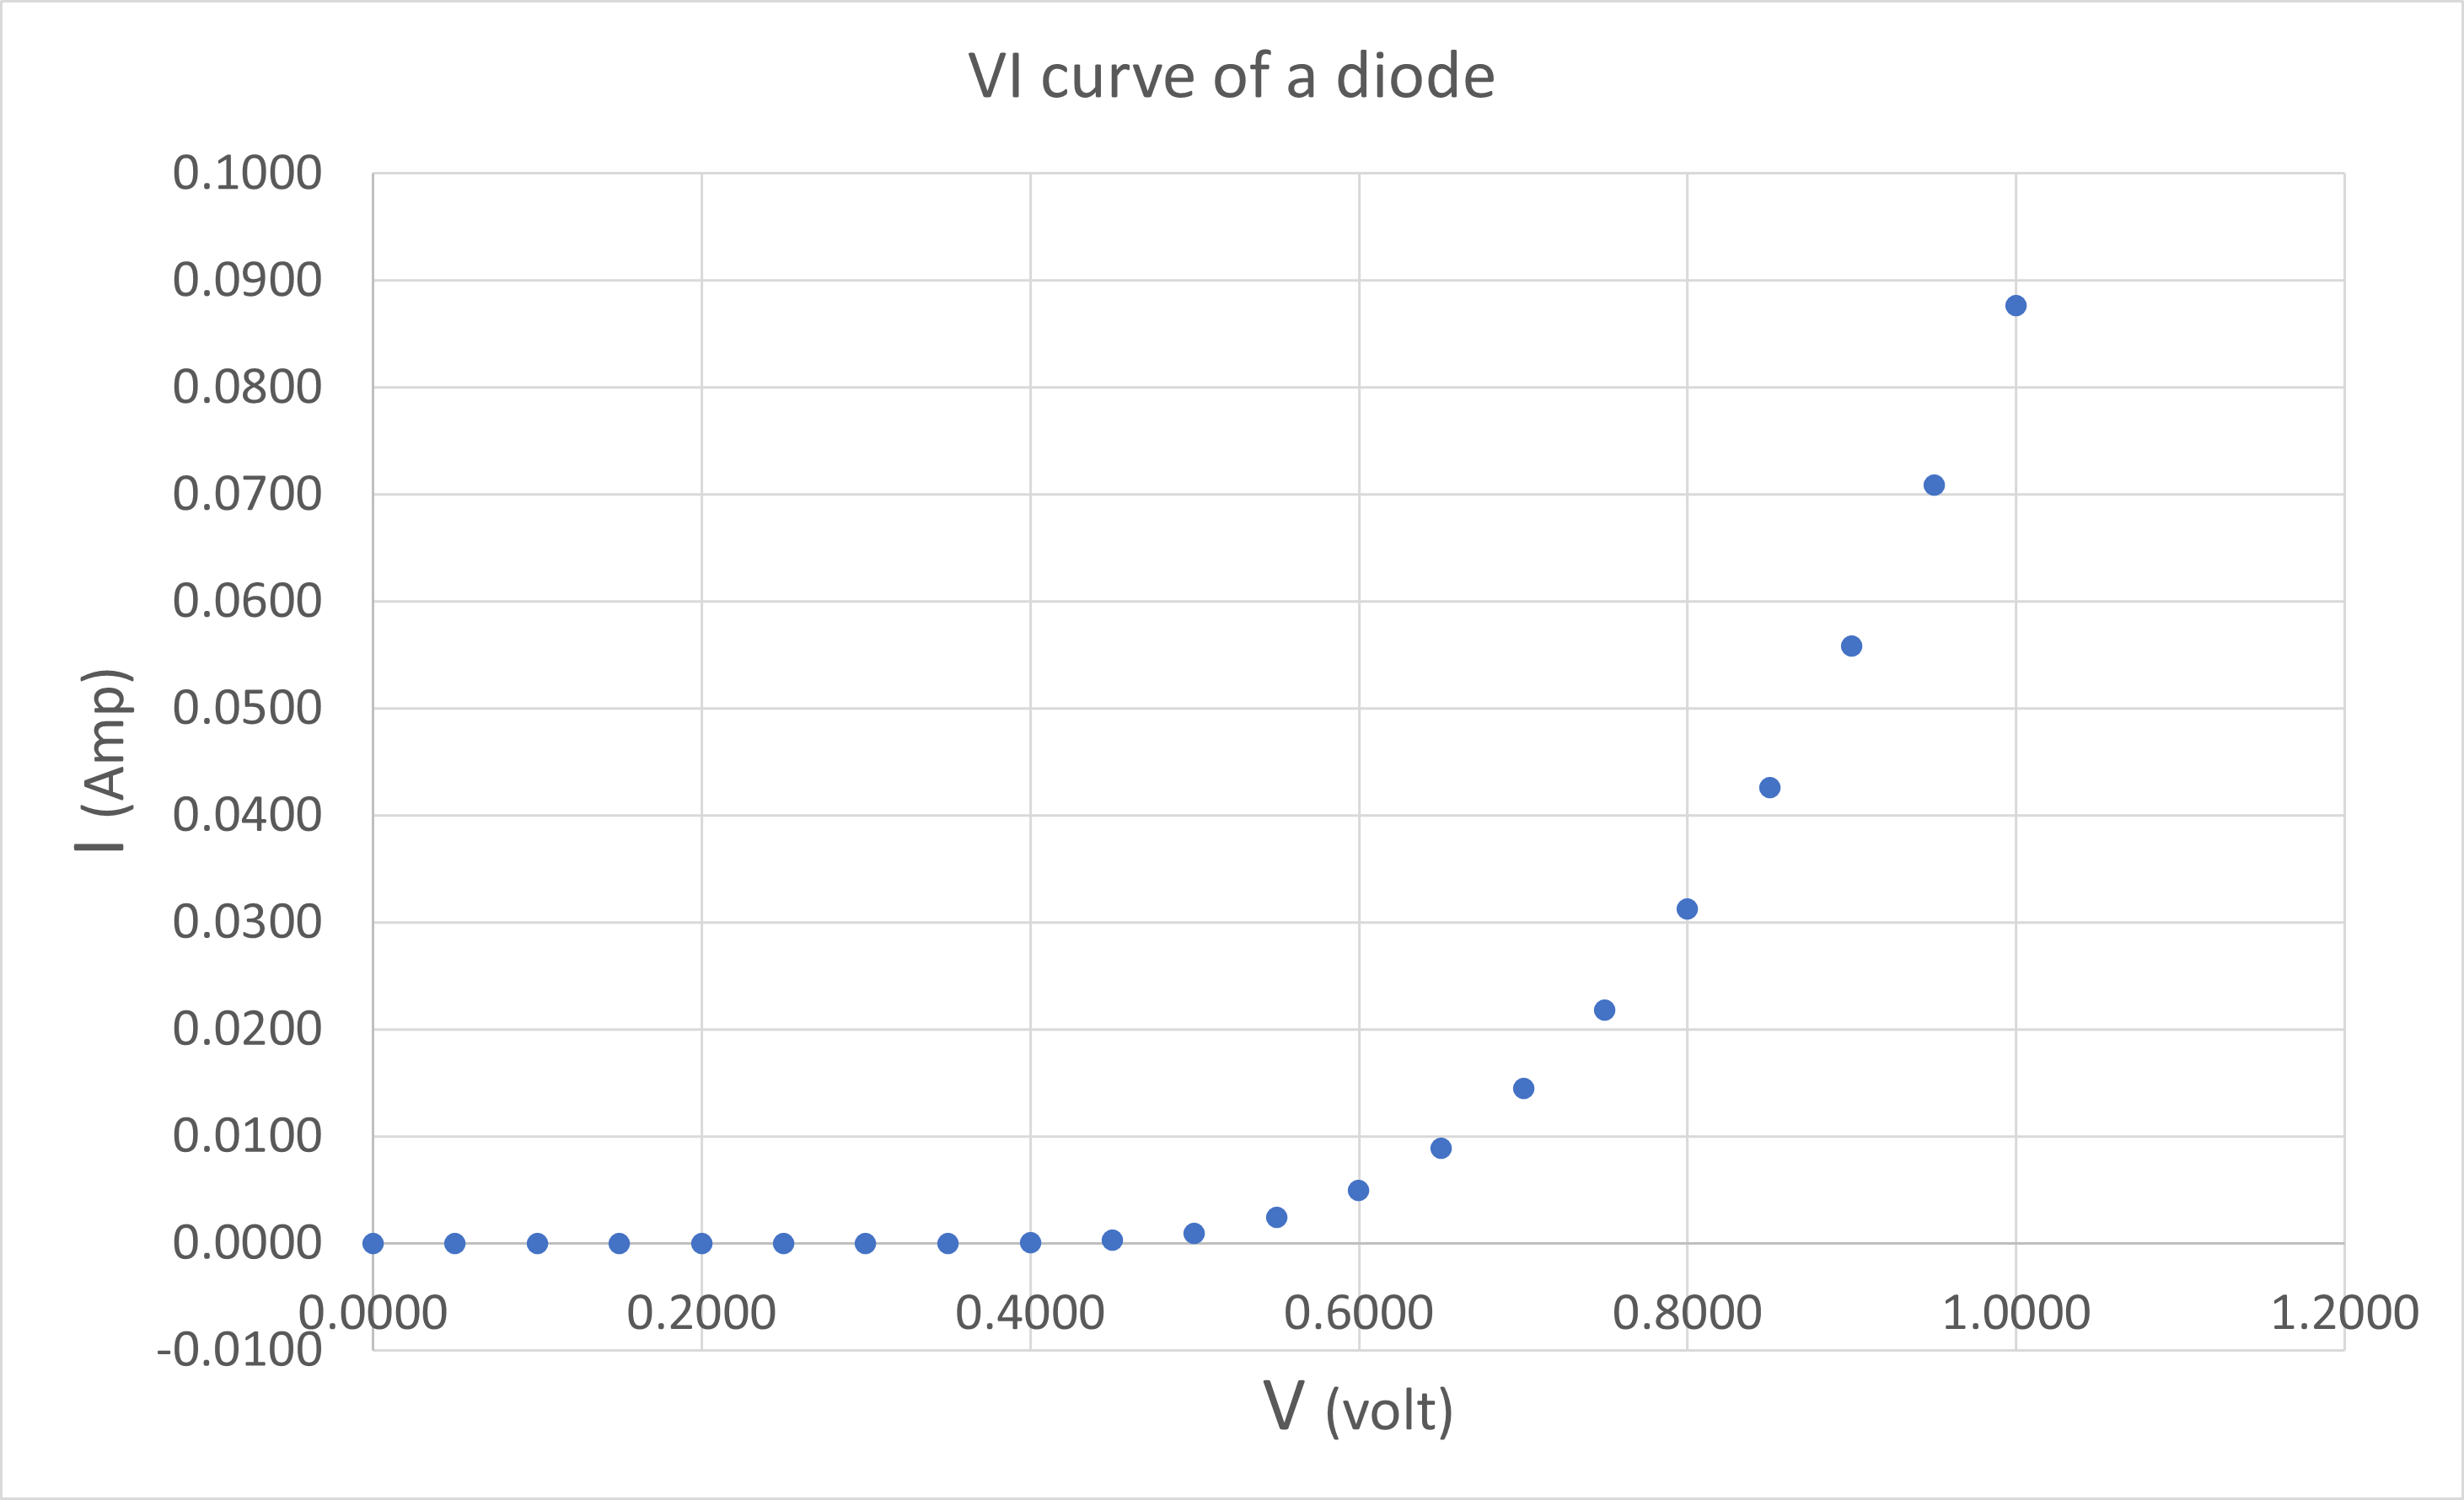
\includegraphics[scale=0.56]{Images/46.png} 
   \caption{Power supply diode automation}
   %\end{subfigure}
\end{figure}
\begin{figure}[H]
%\begin{subfigure}
	\centering
   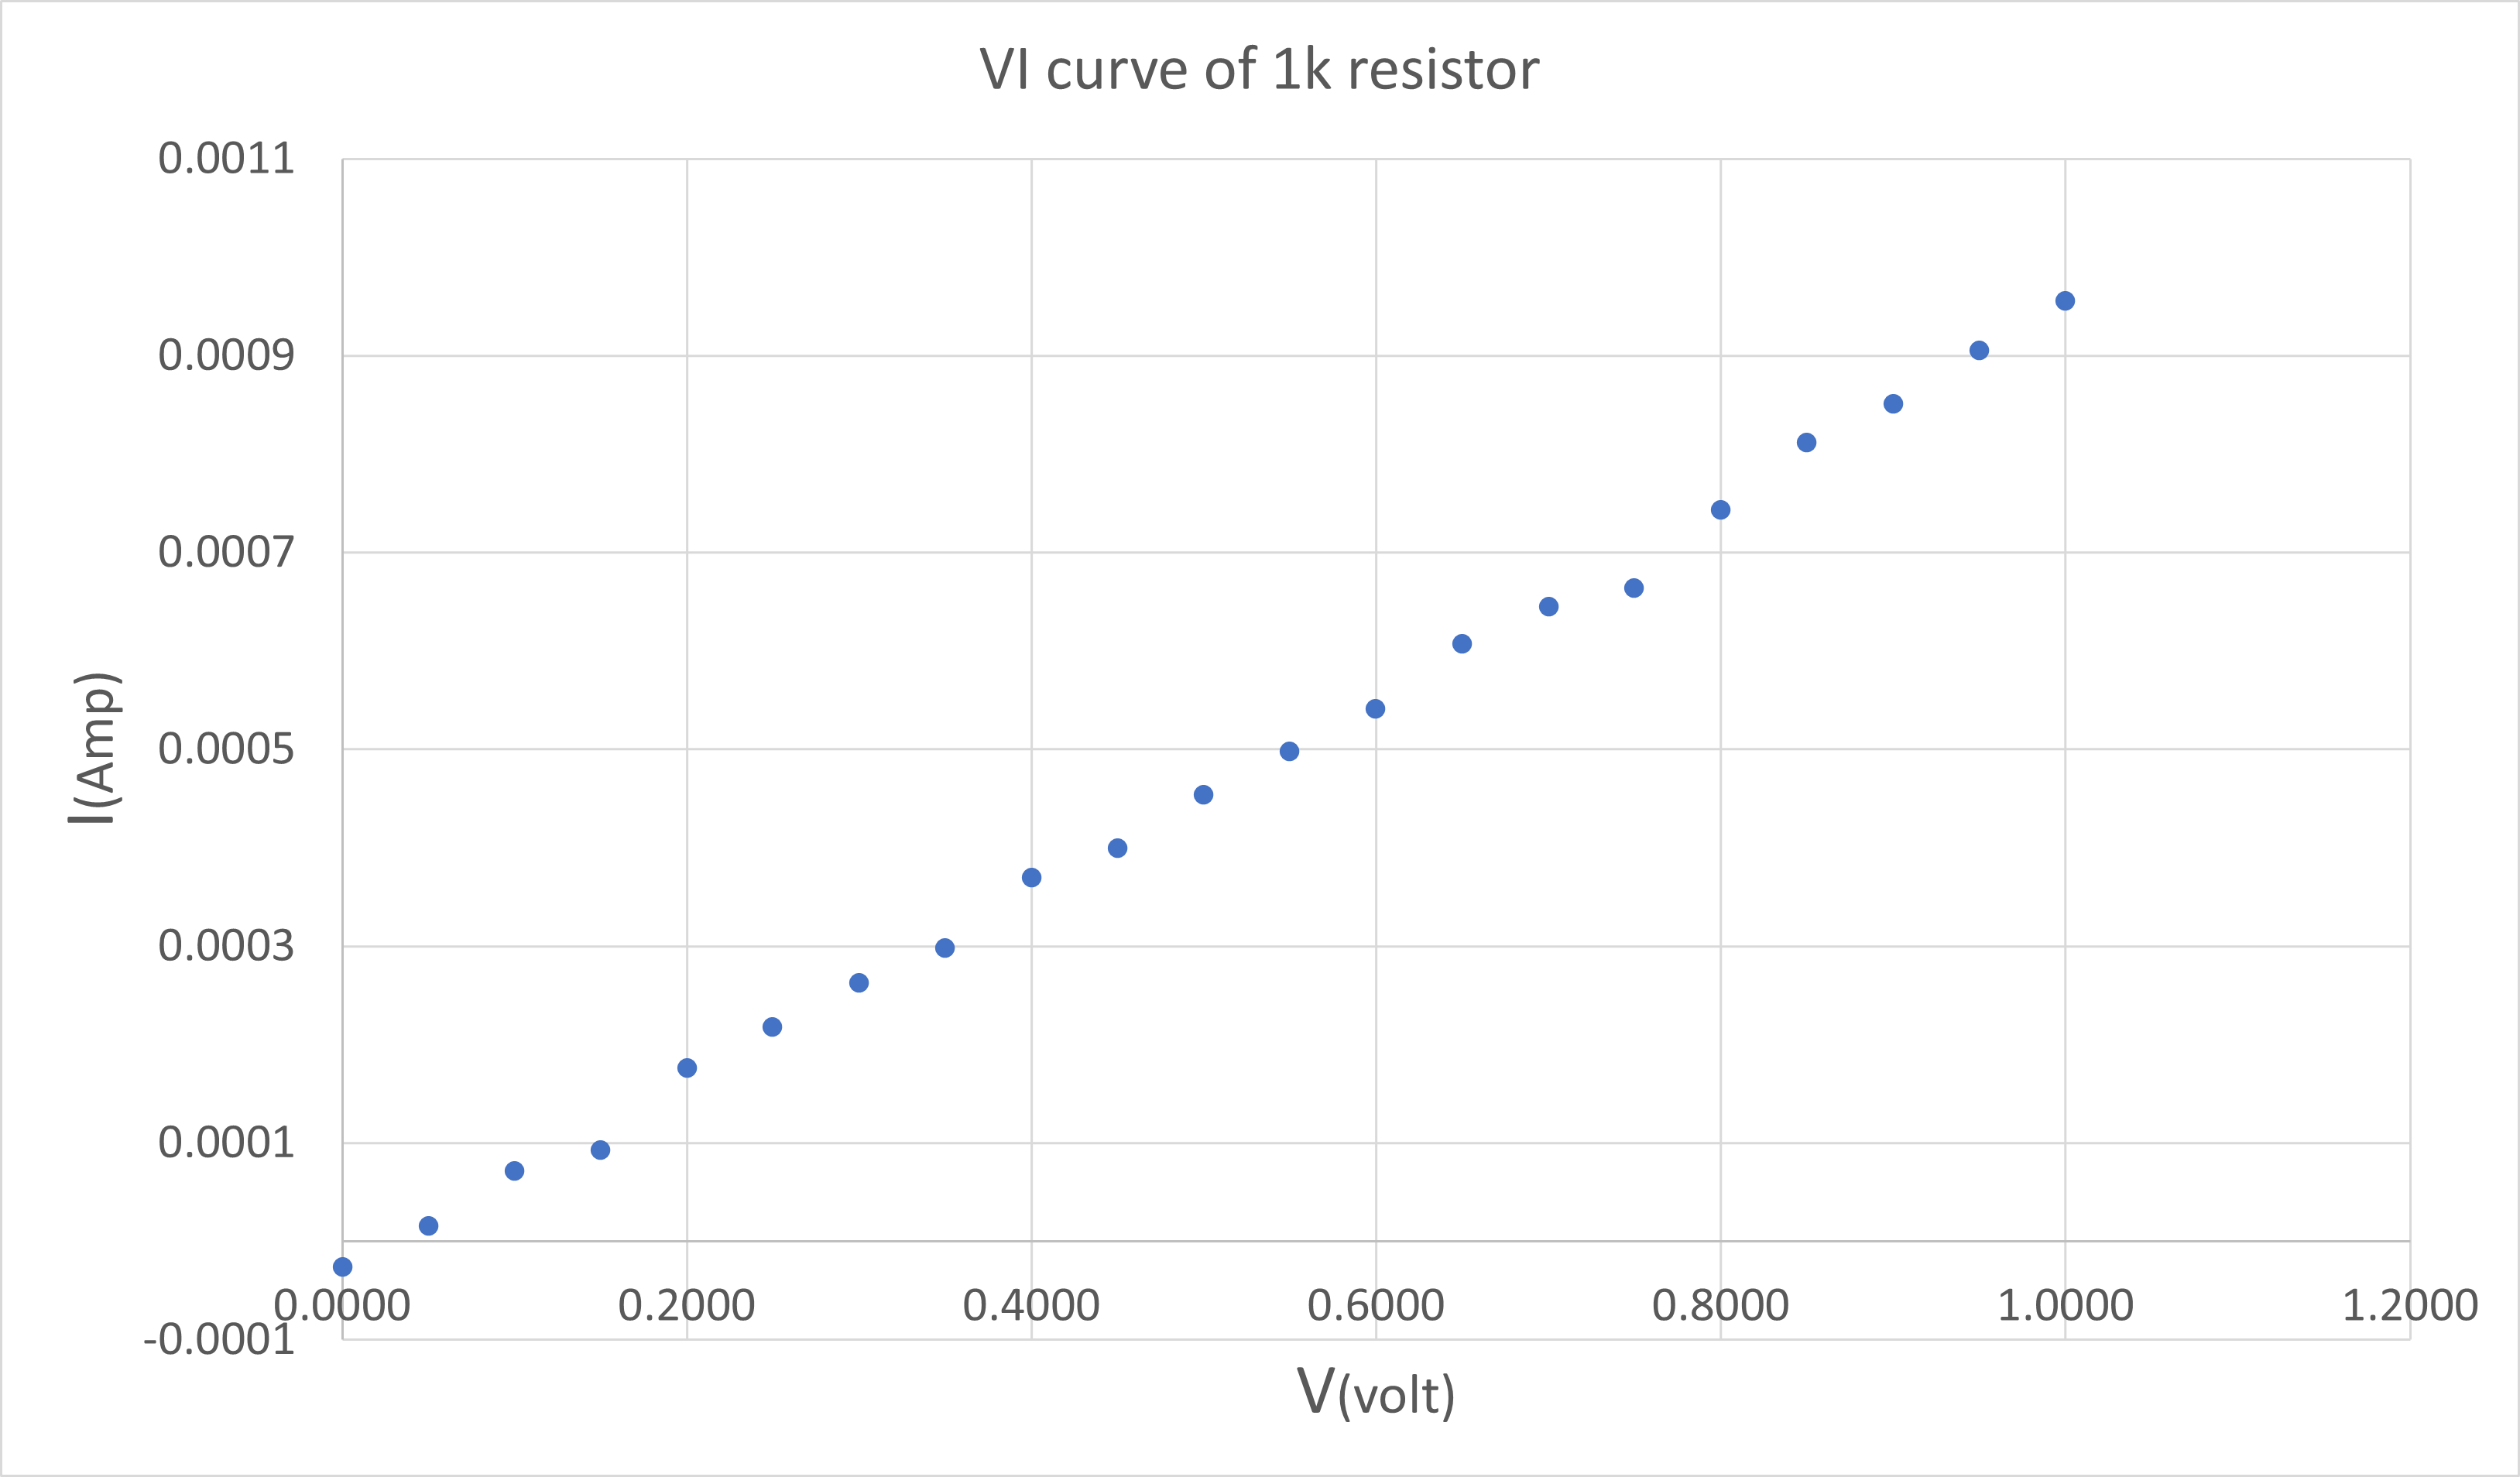
\includegraphics[scale=0.56]{Images/47.png} 
   \caption{Power supply resistance automation}
   %\end{subfigure}
\end{figure}
\begin{figure}[H]
%\begin{subfigure}
	\centering
   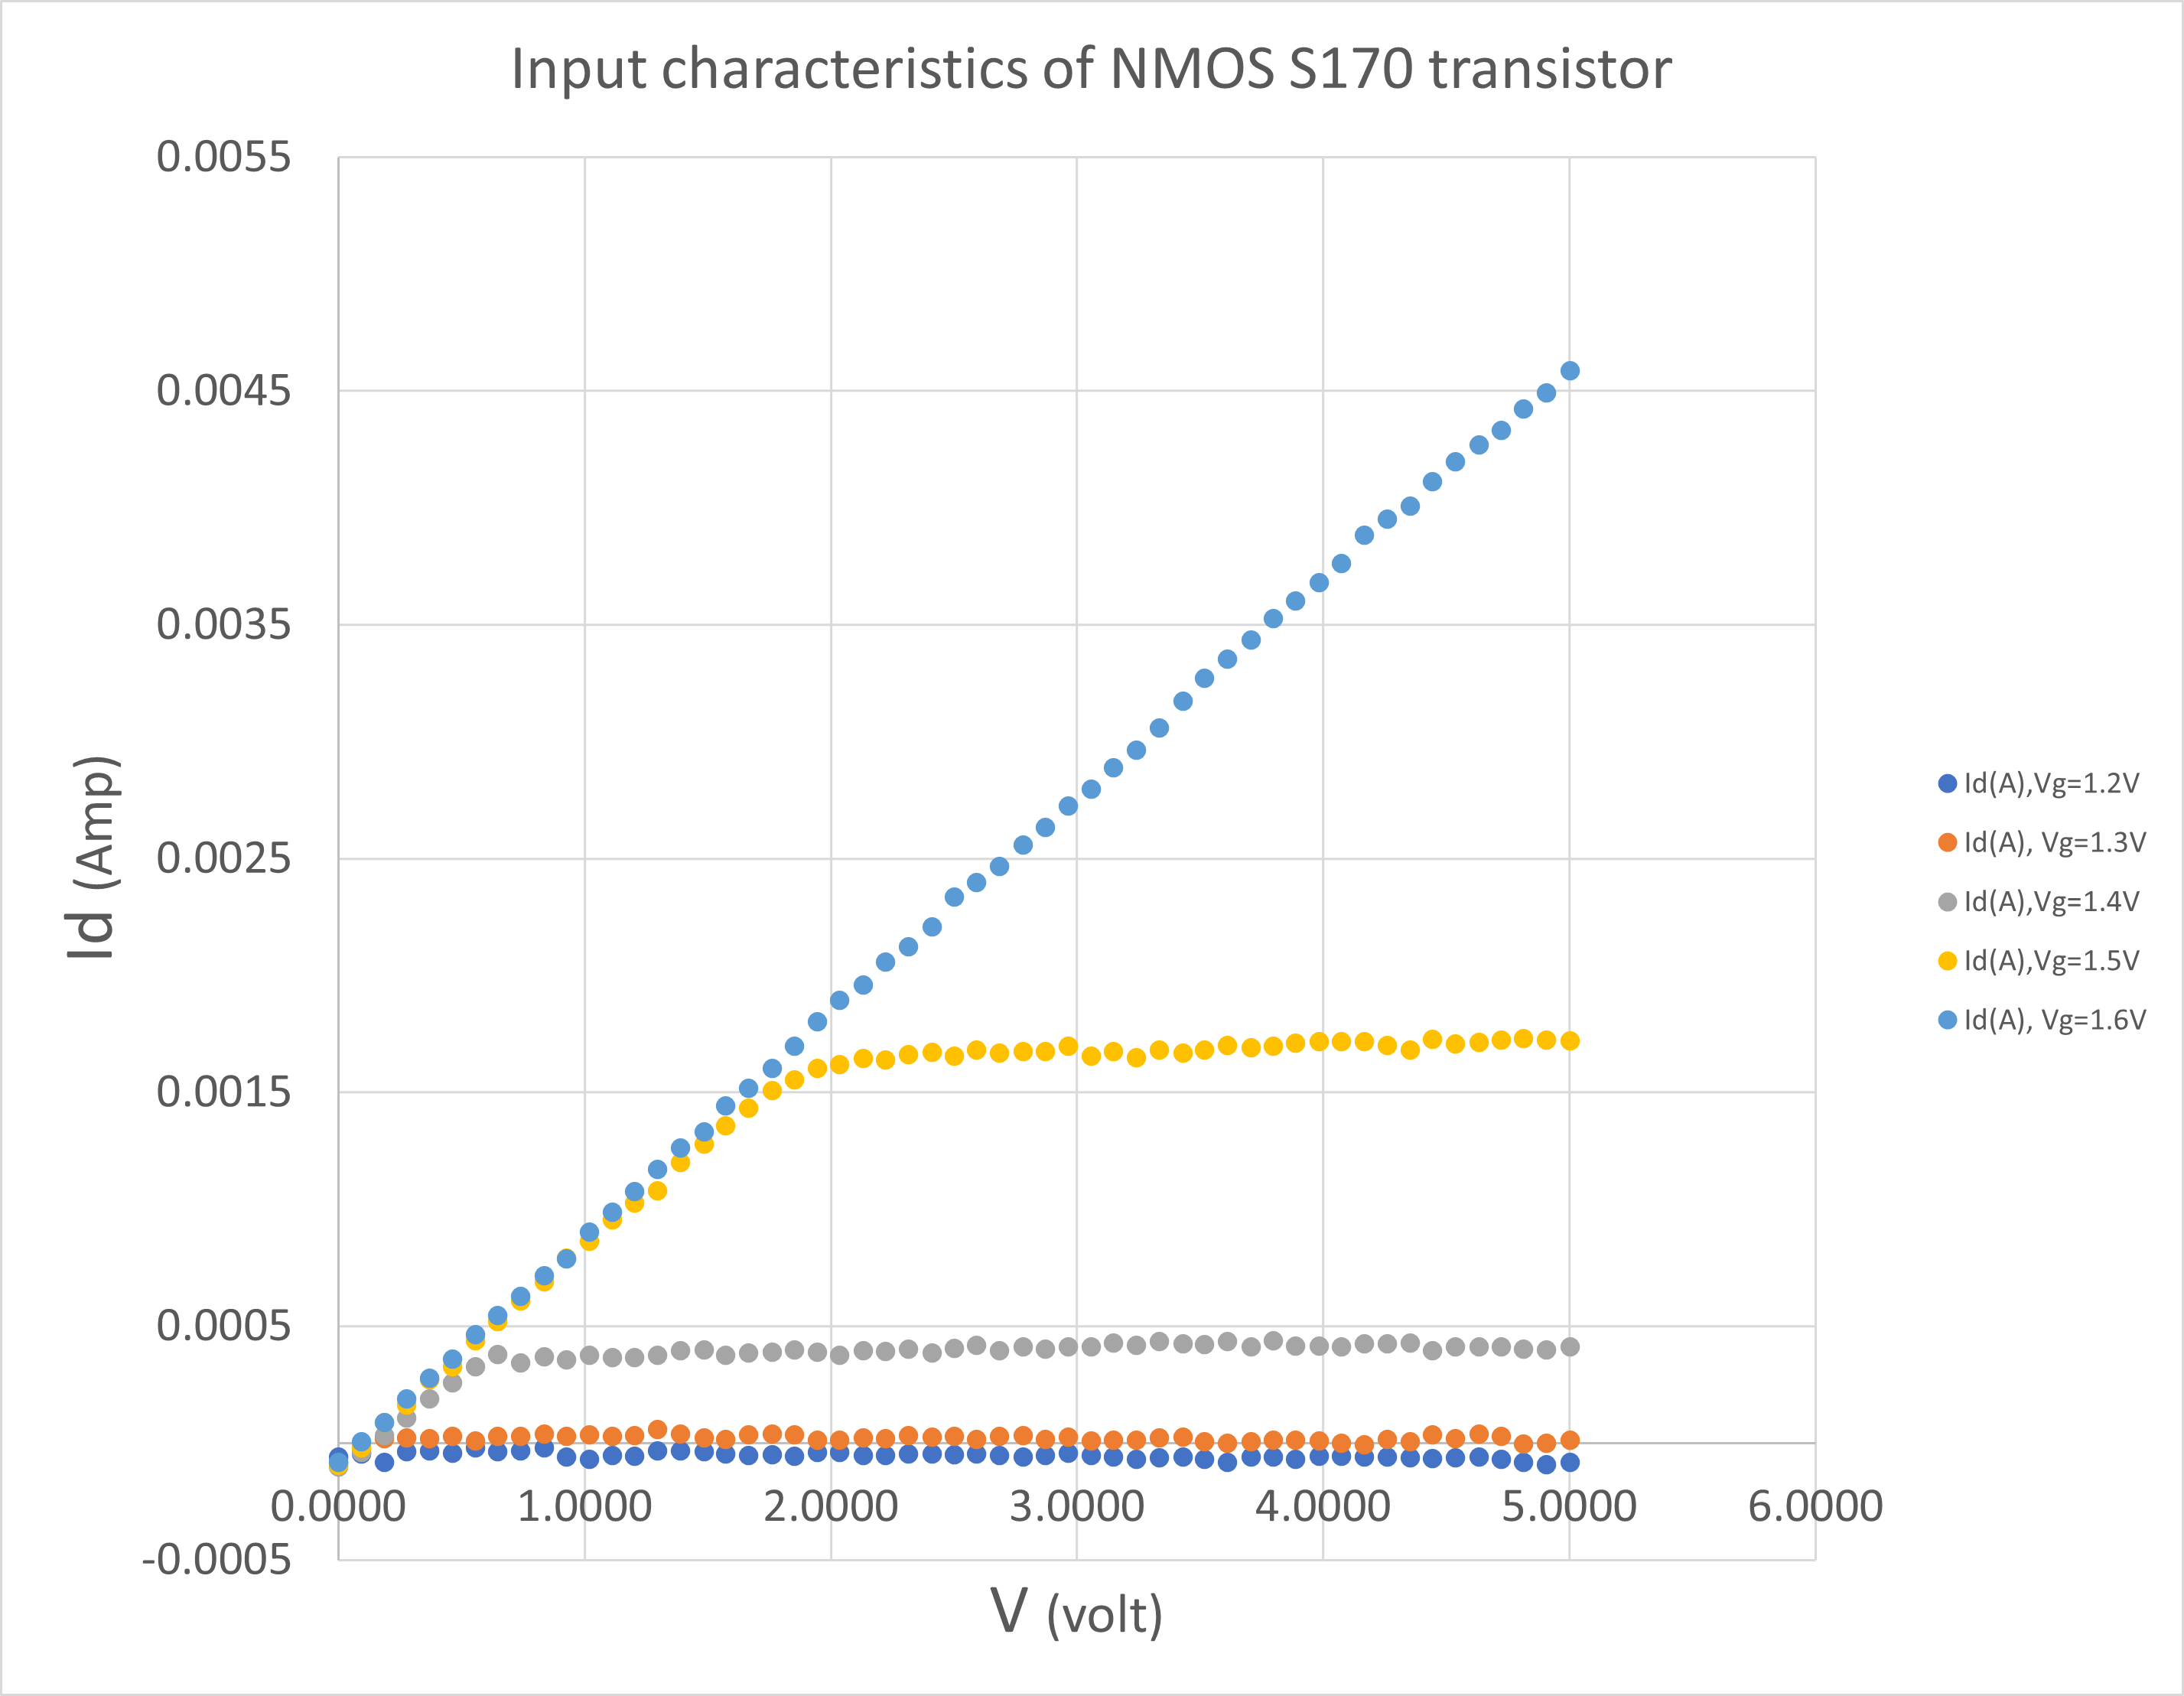
\includegraphics[scale=0.56]{Images/48.png} 
   \caption{Power supply transistor automation}
   %\end{subfigure}
\end{figure}
\subsection{Electromagnet}
\begin{figure}[H]
%\begin{subfigure}
	\centering
   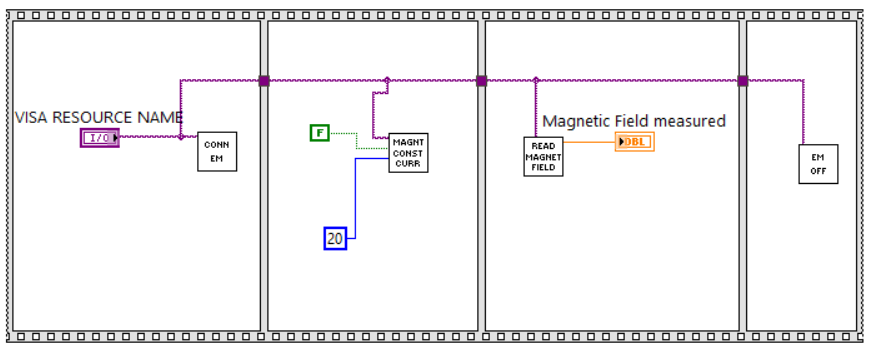
\includegraphics[scale=0.56]{Images/49.png} 
   \caption{LabVIEW: Electromagnet automation}
   %\end{subfigure}
\end{figure}
The electromagnet was automated using LabVIEW. It was used to control the current flowing into the electromagnet's coil to change the constant magnetic field generated at the poles. It was also used to measure the magnetic field through a gauss probe connected to the controller of the electromagnet.
\subsection{Signal generator}
\begin{figure}[H]
%\begin{subfigure}
	\centering
   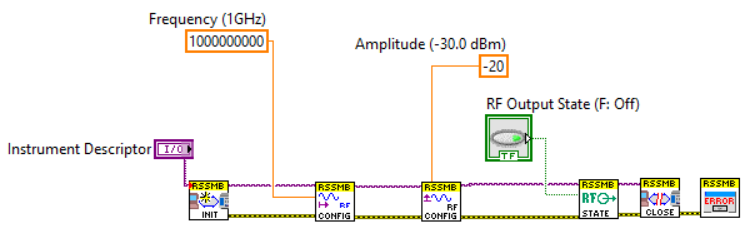
\includegraphics[scale=0.56]{Images/50.png} 
   \caption{LabVIEW: Signal generator automation}
   %\end{subfigure}
\end{figure}
The signal generator was automated using LabVIEW. It was used to set different RF and LF frequencies of different amplitudes. With LabVIEW, the signal generator was automated to sweep from one frequency range to another frequency range.
\subsection{Spectrum analyzer}
\begin{figure}[H]
%\begin{subfigure}
	\centering
   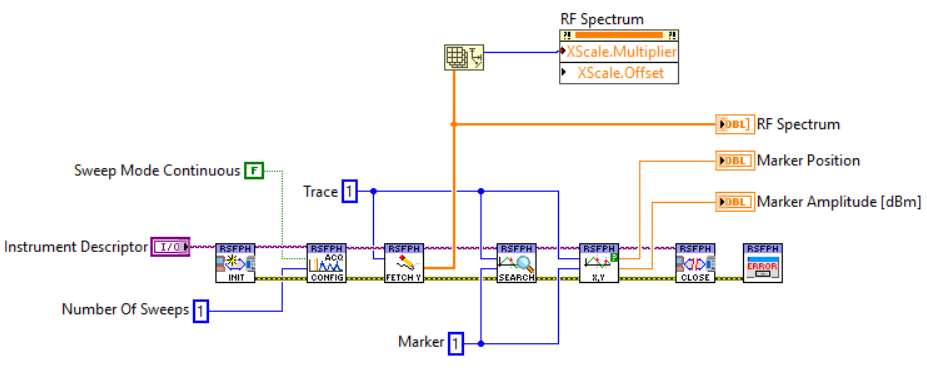
\includegraphics[scale=0.56]{Images/51.png} 
   \caption{LabVIEW: Spectrum analyzer automation}
   %\end{subfigure}
\end{figure}
The spectrum analyzer was automated using LabVIEW to measure the power level of a given input signal. It was able to program the device, where to put the marker, setting the center frequency.
\subsection{Lock-in amplifier}
\begin{figure}[H]
%\begin{subfigure}
	\centering
   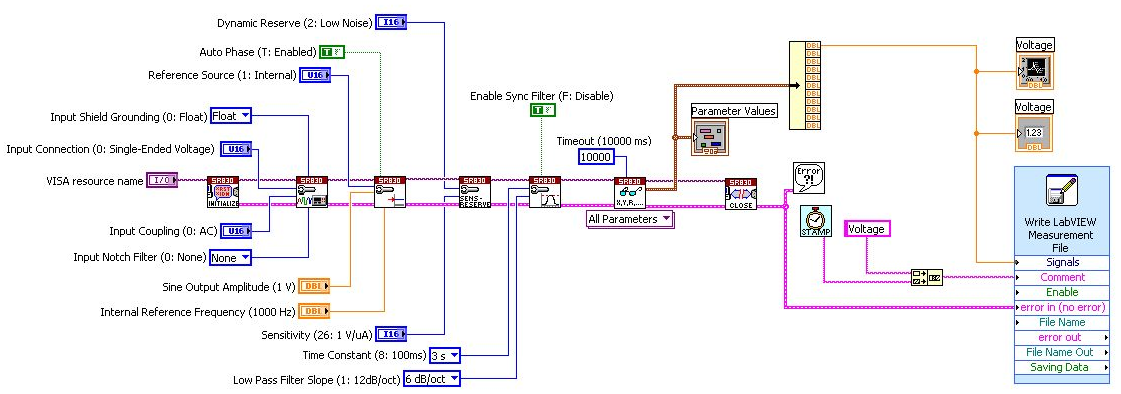
\includegraphics[width=12cm]{Images/45.png} 
   \caption{LabVIEW: Lock-in amplifier automation}
   %\end{subfigure}
\end{figure}
The Lock-in amplifier was automated using LabVIEW to remove noise from a signal by narrowing the bandwidth. It was automated to take single or differential mode input, setting up the sensitivity and the time constant, Etc. Apart from this, it can directly program the lock-in amplifier to set an internal reference frequency
\section{Development of Ferromagnetic resonance system}
The ferromagnetic resonance setup consists of an electromagnet, signal generator, spectrum analyzer, waveguide, and a laptop/pc with LabVIEW.
The magnetic sample is placed on top of the waveguide's signal channel. For in-plane ferromagnetic resonance, the longer side of the sample is placed in parallel to the signal line. The waveguide, along with the sample, is placed in between the poles of the electromagnet. The electromagnet generates the DC magnetic field, which creates the precessing of the magnetization vector. To negative the damping of the magnetization vector, a transverse AC field is required, provided by the signal generator, connected to the input end of the waveguide. The output from the waveguide is fed into the spectrum analyzer to measure the FMR absorption. 
\subsection{Characteristic impedance of coaxial cable}
If the coaxial cable is terminated with a purely resistive load, R, the signal will be reflected or transmitted at the end of the line. The transmission coefficient, T is given by:
\[T=\frac{2R}{R+Z_{cable}}\]
where 
\[T=\frac{V_t}{V_0}=\frac{\text{transmitted signal}}{\text{insident signal}}\]

In a limiting case, if the resistive load is infinite, the transmission coefficient becomes 2, i.z. The transmitted pulse is twice the incident pulse,
\[\text{if R}\rightarrow\infty\text{; T=2;}V_t=2V+0 \]
 and if the resistive load is equal to the Zcable,  the transmission coefficient becomes 1, i.z. The transmitted pulse is same as the incident pulse.
\[\text{if R}\rightarrow Z_{cable}\text{; T=1;}V_t=2V+0 \]
By adding a potentiometer in parallel, the transmitted signal can be measured as a function of R.
\[\frac{1}{T}=\frac{1}{2} + \frac{Z_{cable}}{2R}\]
The slope of this equation gives the $Z_{cable}$ value.

\begin{center}
\begin{tabular}{||c c c c c c||} 
 \hline
 $V_0$ & $V_t$ & R & T & $\frac{1}{2R}$ & $\frac{1}{T}$\\ [0.5ex] 
 \hline\hline
 1.002 & 0.8340 & 49.8 & 1.66 & 0.00100 & 0.6007\\
 1.002 & 0.9060 & 100.1 & 1.81 & 0.0050  & 0.5530\\
 1.002 & 0.9600 & 200 & 1.92 & 0.0025  & 0.5219\\
 1.002 & 0.9720 & 300 & 1.94 & 0.0017 & 0.5154\\
 1.002 & 0.9800 & 400 & 1.96 & 0.0013 & 0.5112\\
 1.002 & 0.9860 & 500 & 1.97 & 0.0010 & 0.5081\\
 1.002 & 0.9900 & 600 & 1.98 & 0.0008 & 0.5061\\
 1.002 & 0.9940 & 700 & 1.98 & 0.0007 & 0.5040\\
 1.002 & 0.9960 & 800 & 1.99 & 0.0006 & 0.5030\\ 
 1.002 & 0.9980 & 900 & 1.99 & 0.0006 & 0.5020\\
 1.002 & 1.0000 & 1000 & 2.00 & 0.0005 & 0.5010\\ [1ex] 
 \hline
\end{tabular}
\end{center}
\begin{figure}[H]
%\begin{subfigure}
	\centering
   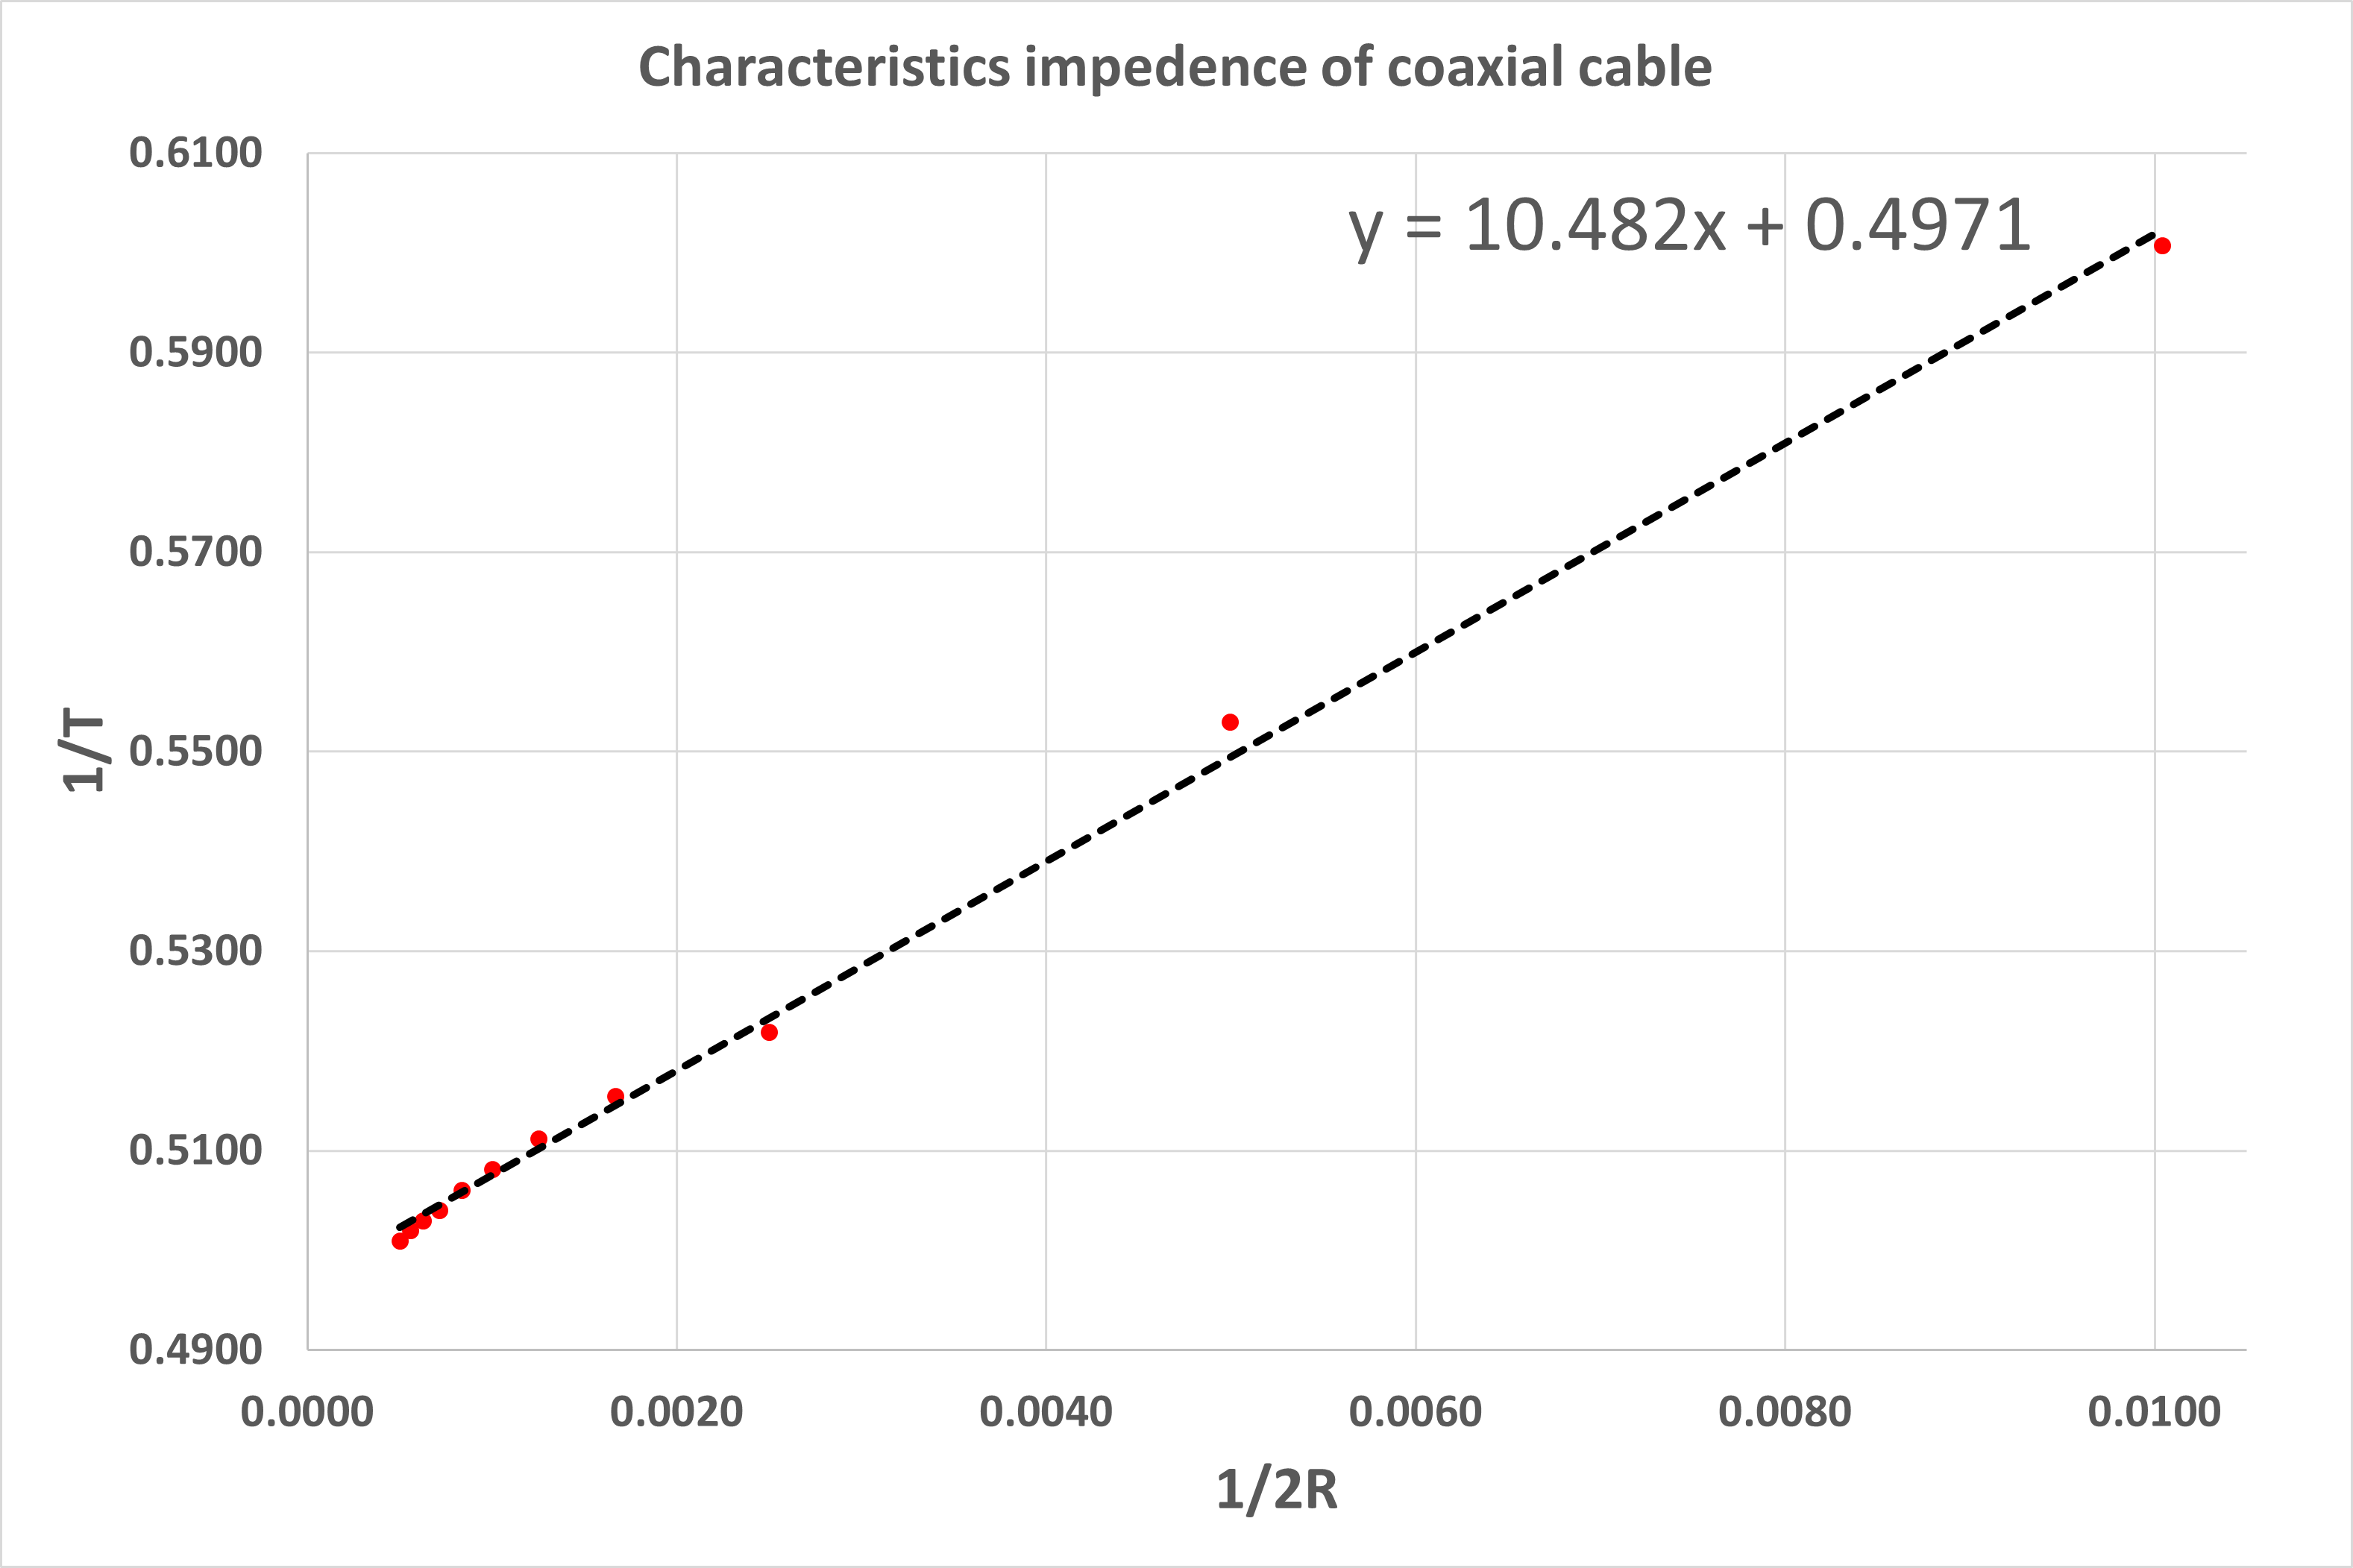
\includegraphics[scale=0.56]{Images/44.png} 
   \caption{Characteristics impedance of coaxial cable}
   %\end{subfigure}
\end{figure}
From the above figure, the fitted linear line gives the $Z_{cable} = 10.482 \Omega$ 
%\subsection{Characteristic impedance of waveguide}
%\subsection{Voltage and current measurement through coaxial cable}
%Mention the oscilloscope results and power level of signal generator
\subsection{Measurement of loss in the coaxial cable, connectors and the waveguide}
Losses in the Coaxial cable and connectors\\
\textbf{Connection 1:} Signal generator is connected to the spectrum analyzer through an SMA cable (Coaxial cable); from here, the loss due to a coaxial cable can be calculated.\\
\textbf{Connection 2:} Signal generator is connected to the waveguide using an SMA cable, and the output from the waveguide is connected to the spectrum analyzer through another SMA cable; from here, the loss due to the waveguide and 2x SMA cable can be calculated.\\ 
\textbf{Connection 3:} Same as Connection 2, with one L-connector connected to the waveguide; from here, the loss due to the waveguide, 2x SMA cable, and the L-connector can be calculated.\\
\textbf{Connection 4:} Same as Connection 3, with one additional T-connector connected to the other end of the waveguide; from here, the loss due to the waveguide, 2x SMA cable, the L-connector, and the T-connector can be calculated.\\
\textbf{Connection 5:} Same as Connection 3, with one additional 50$\Omega$ termination to one open end of the  T-connector; from here, the loss due to the waveguide, 2x SMA cable, the L-connector, the T-connector, and the 50$\Omega$ termination can be calculated.\\\\
The signal generator was connected to the RF port at a frequency of 10 GHz and -10 dBm power
\begin{center}
\begin{tabular}{||c c c c||} 
 \hline
 Connections & Signal generator dbM & Spectrum analyzer dbM & loss (dBm)\\ [0.5ex] 
 \hline\hline
 Connection 1 & -10 & -25.5 & 15.5\\ 
 Connection 2 & -10 & -43 & 33\\
 Connection 3 & -10 & -49 & 39\\
 Connection 4 & -10 & -44 & 34\\
 Connection 5 & -10 & -49.4 & 39.4\\  [1ex] 
 \hline
\end{tabular}
\end{center}
\begin{center}
\begin{tabular}{||c c||} 
 \hline
 Components & Loss(dBm) \\ [0.5ex] 
 \hline\hline
 SMA cables & 15.5 \\ 
 Waveguide & 2 \\
 L-connector & 6 \\
 T-connector & -5 \\
 50 $\Omega$ termination & 5.4 \\  [1ex] 
 \hline
\end{tabular}
\end{center}
\subsection{FMR result}
\begin{figure}[H]
%\begin{subfigure}
	\centering
   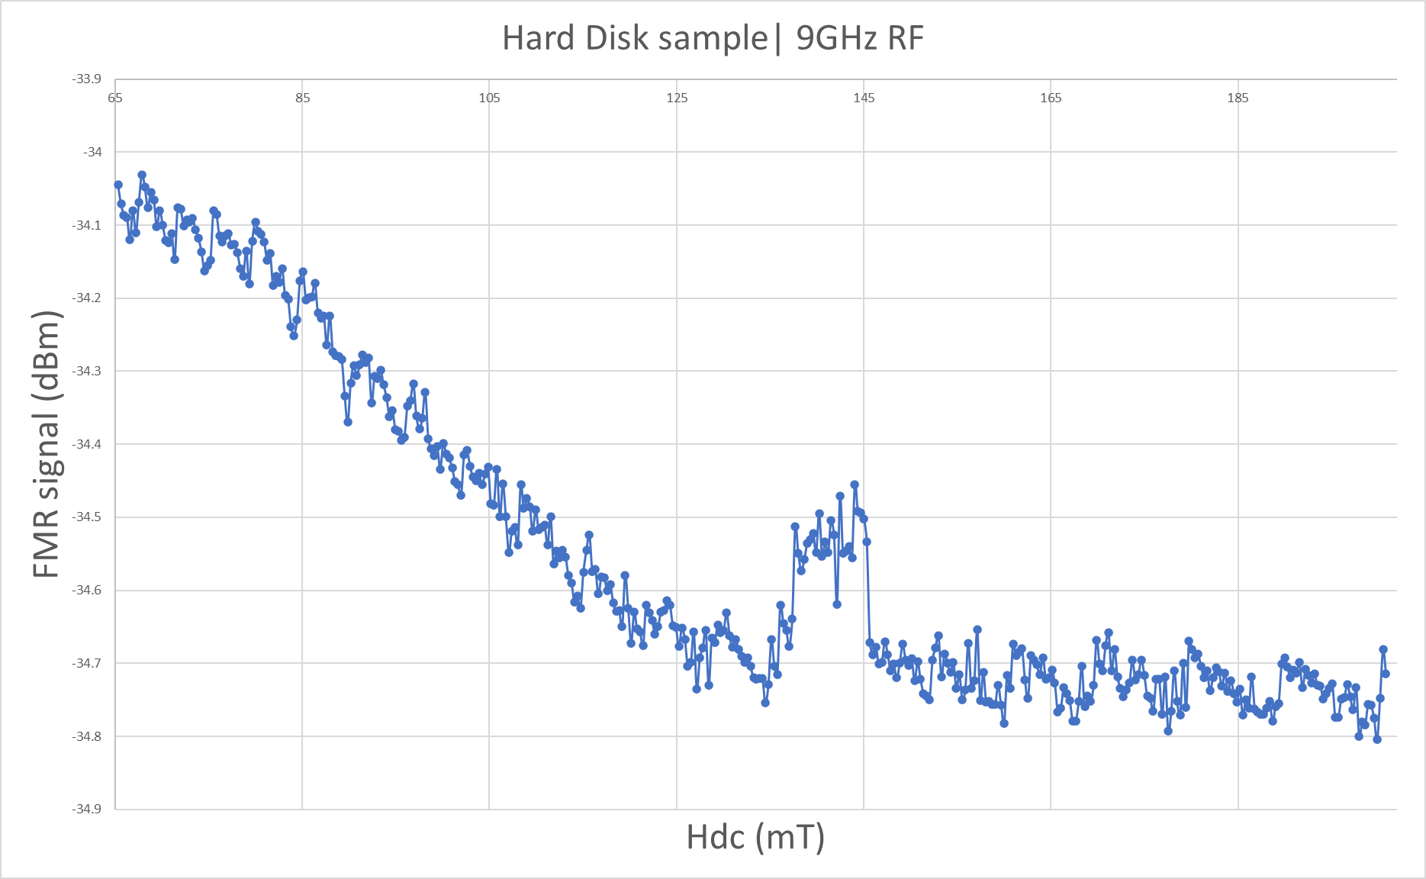
\includegraphics[scale=0.56]{Images/43.png} 
   \caption{FMR result}
   %\end{subfigure}
\end{figure}
\subsection{Schootky diode measurement results}
The frequency of the output signal from the waveguide is in GHz, and the standard diode available can rectify AC signals up to 10 kHz frequency. Hence we use a Schottky diode to rectify the 9 GHz signal. 
\\\\
Schottky diodes are constructed using a metal electrode and N-type material. Since the Schottky diode has a metal electrode on one side, it does not have the depletion region. The junction formed by the metal and the N-type material is the metal-semiconductor junction. The electron from the N-type material goes to the metal electrode in the forward bias. The drift of the majority of carriers enables the current to flow. In reverse bias, since there is no P-type material, there are no minority carriers to form the depletion region. The diode conduction stops very quickly, stopping the current flow.
\\
Two Schottky diodes available in the market were tested, SRP BAT85 and Infineon diode [model name]. The following are the results tested on each diode at a different frequency and power level. \\\\
\textbf{Schottky diode: SRP BAT85 }\\\\
\begin{minipage}[b]{0.48\linewidth}
%\centering
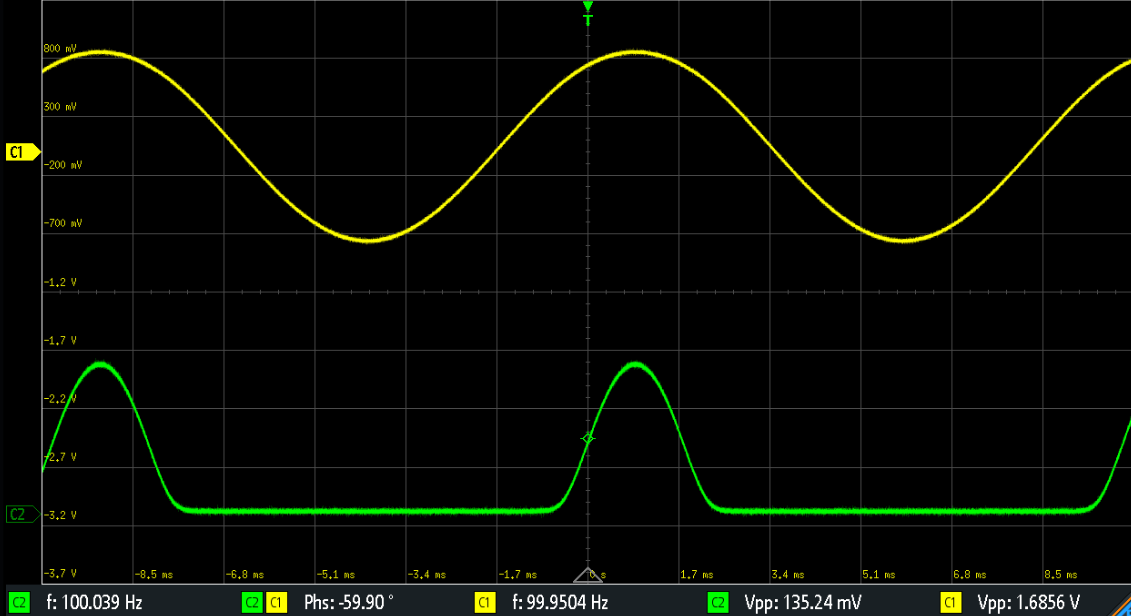
\includegraphics[width=6.7cm]{Images/Amazon/LF100Hz.png}  
Input signal frequency: 100 Hz\\
Signal without rectifying\\
$Vpp = 1.6856\text{ }V$\\
Signal after rectifying\\
$Vpp = 135.24\text{ }mV$\\
\end{minipage}
\hfill
\begin{minipage}[b]{0.48\linewidth}
%\centering
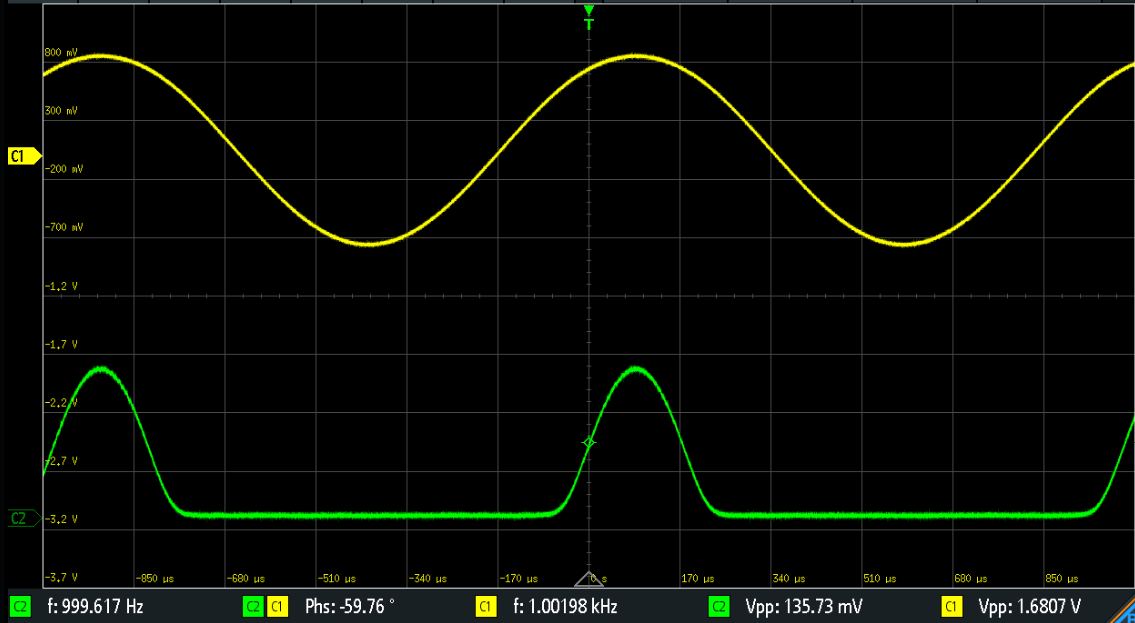
\includegraphics[width=6.7cm]{Images/Amazon/LF1kHz.png}  
Input signal frequency: 1 kHz\\
Signal without rectifying\\
$Vpp = 1.6807\text{ }V$\\
Signal after rectifying\\
$Vpp = 135.73\text{ }mV$\\
\end{minipage}
\\
\begin{minipage}[b]{0.48\linewidth}
%\centering
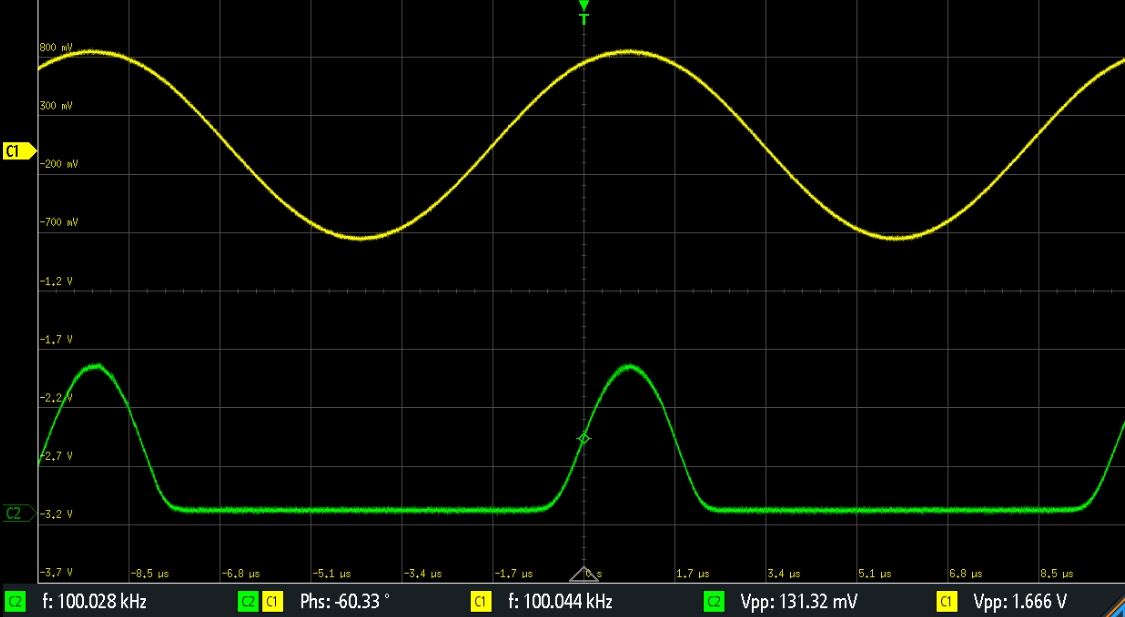
\includegraphics[width=6.7cm]{Images/Amazon/LF100kHz.png}  
Input signal frequency: 100 kHz\\
Signal without rectifying\\
$Vpp = 1.666\text{ }V$\\
Signal after rectifying\\
$Vpp = 131.32\text{ }mV$\\
\end{minipage}
\hfill
\begin{minipage}[b]{0.48\linewidth}
%\centering
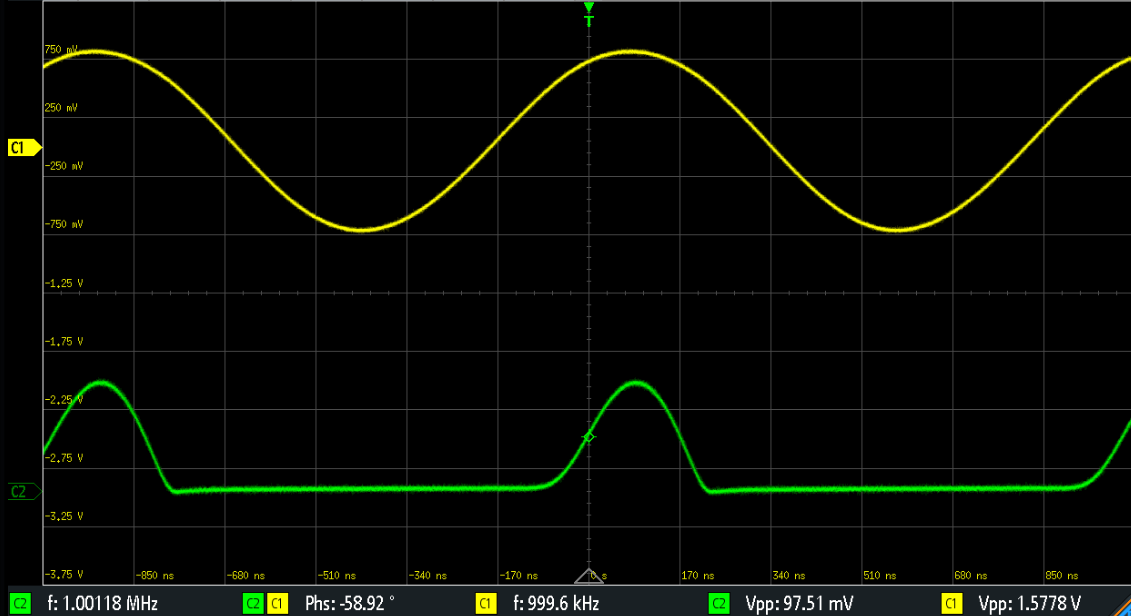
\includegraphics[width=6.7cm]{Images/Amazon/LF1MHz.png}  
Input signal frequency: 1 MHz\\
Signal without rectifying\\
$Vpp = 1.5778\text{ }V$\\
Signal after rectifying\\
$Vpp = 97.51\text{ }mV$\\
\end{minipage}
%-------------------
\\\\
\textbf{Schottky diode: Infineon [model name]}\\\\
\begin{minipage}[b]{0.48\linewidth}
%\centering
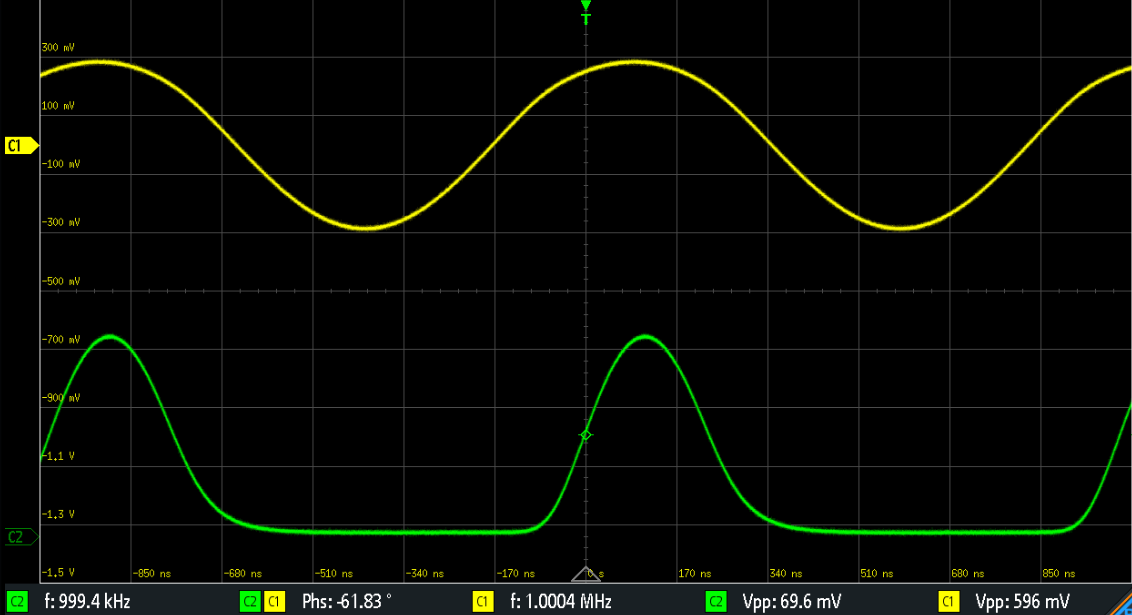
\includegraphics[width=6.7cm]{Images/Infinion/RF1MHz.png}  
Input signal frequency: 100 kHz\\
Signal without rectifying\\
$Vpp = 596\text{ }mV$\\
Signal after rectifying\\
$Vpp = 69.6\text{ }mV$\\
\end{minipage}
\hfill
\begin{minipage}[b]{0.48\linewidth}
%\centering
\includegraphics[width=6.7cm]{Images/Infinion/RF5MHz.png}  
Input signal frequency: 1 MHz\\
Signal without rectifying\\
$Vpp = 558\text{ }mV$\\
Signal after rectifying\\
$Vpp = 47.8\text{ }mV$\\
\end{minipage}
\\
\begin{minipage}[b]{0.48\linewidth}
%\centering
\includegraphics[width=6.7cm]{Images/Infinion/RF10MHz.png}  
Input signal frequency: 100 kHz\\
Signal without rectifying\\
$Vpp = 542\text{ }mV$\\
Signal after rectifying\\
$Vpp = 25.088\text{ }mV$\\
\end{minipage}
\hfill
\begin{minipage}[b]{0.48\linewidth}
%\centering
\includegraphics[width=6.7cm]{Images/Infinion/RF20MHz.png}  
Input signal frequency: 1 MHz\\
Signal without rectifying\\
$Vpp = 429.24\text{ }mV$\\
Signal after rectifying\\
$Vpp = 20.139\text{ }mV$\\
\end{minipage}
\\
\begin{minipage}[b]{0.48\linewidth}
%\centering
\includegraphics[width=6.7cm]{Images/Infinion/RF50MHz.png}  
Input signal frequency: 100 kHz\\
Signal without rectifying\\
$Vpp = 490\text{ }mV$\\
Signal after rectifying\\
$Vpp = 25.284\text{ }mV$\\
\end{minipage}
\hfill
\begin{minipage}[b]{0.48\linewidth}
%\centering
\includegraphics[width=6.7cm]{Images/Infinion/RF100MHz.png}  
Input signal frequency: 1 MHz\\
Signal without rectifying\\
$Vpp = 201.88\text{ }mV$\\
Signal after rectifying\\
$Vpp = 66\text{ }mV$\\
\end{minipage}
\section{Sputtering deposition}
Before fabricating the device, it is needed to calibrate the parameters of the multiferroics, such as damping parameter $\alpha$, $d_{33}$ and so on. Hence depositing thin films are an inexpensive way to do so.\\
Deposition of Kapton can be used as a substrate for the thin film since it is flexible and can endure high temperatures. PMN-PT (Lead Magnesium Niobate-Lead Titanate) is used for piezoelectric and magnetostrictive material, FeGa.\\
All deposition is from the substrate side, and all the numbers inside the bracket are the nominal thickness in nm.\\\\
Thin-film 1\\
Kapton/PMN-PT(25, 50, 75, 100)\\
From this thin film, for different thicknesses of PMN-PT, the $d_{33}$, Young's modulus, Poisson ratio, and d-coefficient can be calculated.\\\\
Thin-film 2\\
Kapton/PMN-PT(25, 50, 75, 100)/FeGa(0.8, 1, 1.5, 1.7, 2, 5, 10, 20, 50, 100)\\
From this thin film, for different thicknesses of PMN-PT and FeGa, the damping parameter $\alpha$ can be calibrated by obtaining the MH hysteresis, the saturation magnetization, and the coercive field is calculated.\\\\
Thin-film 3\\
Kapton/PMN-PT(50)/FeGa(2)/$Al_2O_3$(40)/CoFeB(2)MgO(0.8)/CoFeB(2)/\\Ta(5)/Ru(5)/Cr or Au\\
This thin film suggests the entire stack, which can be used as one single neuron. Here we have the multiferroic, and on top of that, we have the TMR.\\\\
Thin-film 4\\
Kapton/PMN-PT(50)/FeGa(2)/MgO(0.8)/CoFeB(2)/Ta(5)/Ru(5)/Cr or Au\\
This thin film is a modification of the thin-film 3, and here it is tried to get the TMR property in between FeGa and CoFeB using a MgO spacer, thereby reducing the stack into a compact version.\\\\
Thin-film 5\\
Kapton/PMN-PT(50)/FeGa(2)/MgO(0.8)/CoFeB(2)\\
This thin film is the same as Thin-film 4, except for the outer metallic contact layer to visualize the magnetization of the top CoFeB layer by MFM.
\begin{figure}[H]
%\begin{subfigure}
	\centering
   \includegraphics[width=13cm]{Images/52.png} 
   \caption{Sputtering thin-film deposition}
   %\end{subfigure}
\end{figure}
%\section{EBL patterning}
\section{Neuromorphic devices using multiferroics}
\subsection{Multiferroics}
For a thin-film deposition, we have chosen Lead magnesium niobate-lead titanate (PMN-PT) as piezoelectric material and Iron-galium (FeGa) as magnetostrictive material. FeGa is deposited on PMN-PT. A voltage of 50 mV is applied across the deposition. It creates strain on the piezoelectric material.
\[\epsilon_{piezo}=d_{piezo}\times \frac{V_{in}}{t_{piezo}}\]
where $d_{piezo}$=3000 pm/V for PMN-PT, $t_{piezo}$=100 nm.
The strain is elestically transfered to the magnetostrictive material. 
\[\epsilon_{mag}=\epsilon_{piezo}\] 
Which creates stress anisotropy in the FeGa, stress, $\sigma=Y\epsilon_{mag}$, Young's modulus of FeGa, Y=$250\times 10^9 Pa$
\[\text{Stress anisotropy (FeGa)}=\frac{3}{2}\lambda \sigma \Omega cos^2 \theta=2.4 \times 10^{-18} J\]
\subsection{Read unit using tunnelling junctions}
The stress anisotropy generated from the PMN-PT/FeGa multilayer should be able to reduce the energy barrier of the nanomagnet of the TMR for magnetization switching. As a result, the TMR parallel and anti-parallel orientation are possible.\\
The resistance area product of the parallel orientation of a TMR,
\[R_PA=175 k\Omega \mu m^2\]
$R_P$ is the resistance of TMR when both the magnets are in the parallel direction, and the desired TMR value is 200\%.
\[TMR=\frac{R_{AP}}{R_P}-1\]
hence $R_{AP}=3R_P$
\[R_{AP}A=525 k\Omega \mu m^2\] 
If a constant current, $I_{read}=1 nA$ is given to the TMR of area 100 nm $\times$ 100 nm
\[V_P=I_{read}\cdot \frac{R_PA}{A}=17.5 mV\]
\[V_{AP}=I_{read}\cdot \frac{R_{AP}A}{A}=52.5 mV\]
That is to make the TMR in parallel orientation, 17.5 mV is required and to make anti-parallel orientation, 52.5 mV is required.

\subsection{Device architecture} 
\begin{figure}[H]
%\begin{subfigure}
	\centering
   \includegraphics[width=13cm]{Images/56.png} 
   \caption{Single neuron architecture}
   %\end{subfigure}
\end{figure}
A single neuron of the device consists of the piezoelectric layer, on top of which there are many pillars. These pillars are made up of magnetostrictive material, and on top of the magnetostrictive material, there is a TMR. The pillars are of different areas. The input is given at the piezoelectric layer, and this generates the strain, which is transferred to the magnetostrictive material present in the pillars. The stress anisotropy in the magnetostrictive material affects the energy barrier of the TMR magnet, causing parallel and anti-parallel orientation. In this architecture, the piezoelectric material serves the purpose of summation block~\cite{roy13x}, as if two voltage inputs are given, it will generate strain based on the two inputs. The TMR serves the purpose of the weight of edges. Therefore as many neurons are connected to this neuron, that many numbers of pillars will be there on the piezo material.

\begin{figure}[H]
%\begin{subfigure}
	\centering
   \includegraphics[width=13cm]{Images/57.png} 
   \caption{Neural network hardware}
   %\end{subfigure}
\end{figure}
In the figure, the neural network hardware architecture is compared with an abstract neural network. The abstract network has one neuron in the input layer, two hidden neurons in the hidden layer, and two in the output layer. All the edges connecting to the neurons have weight $W_1, W_2, W_3, W_4, W_5, W_6$. $X_1$ is the input given to the network, and $Y_1, Y_2$ are the network's output.
In the hardware architecture, the weight of the edges is encoded into the pillars. 
\chapter{Conclusions and discussions} \label{ch: conclusions}
To achieve higher cognitive functions like the human brain, mimicking the brain's neural architecture is the ultimate solution for neuromorphic computing. Designing this neuromorphic chip using a multiferroic device gives the extra advantage of being energy-efficient. These devices are endurable in nature; hence these are also best suited for outer space programs. \\
For the multiferroic layer, PMN-PT and FeGa are used, which makes the device more energy-efficient as the de-coefficient of the PMN-PT and magnetoelastic coefficient of FeGa are very high.\\
For improving and stabilizing the magnetization of the magnetic material, magnetic thermal annealing is the best technique.\\
For reducing the TMR lateral dimension, perpendicular anisotropy is used, which even contributes to energy efficiency as perpendicular anisotropy requires very low energy for magnetization switching.\\
By implementing the neuromorphic hardware design, an energy-efficient application-specific neuromorphic hardware can be designed.
% -----------------------------
%\section{Observations}



% -----------------------------
\begin{appendices}
\renewcommand{\thesection}{\Roman{section}}
\section{Basic Definitions}

This is the first section of the appendix.

\section{Additional Theorems}

This is the second section of the appendix.

\end{appendices}
% -----------------------------
\bibliographystyle{plain}
\bibliography{mybib}
\addcontentsline{toc}{chapter}{Bibliography}

\end{document}